
\documentclass[11pt]{article}

% ------------------------------------------------------------
% Standard LaTeX packages
% ------------------------------------------------------------
\usepackage[margin=1in]{geometry}
\usepackage{lmodern}
\usepackage{amsmath,amssymb,mathtools}
\usepackage{amsthm}
\usepackage[american]{babel}
\usepackage{enumitem}
\usepackage{booktabs}
\usepackage{array}
\usepackage{url}
\usepackage{listings}
\usepackage[x11names,table]{xcolor}
\usepackage{tikz}
\usetikzlibrary{positioning,arrows.meta,shapes.geometric,calc,decorations.pathreplacing,patterns}
\usepackage[colorlinks=true,linkcolor=blue,citecolor=blue,urlcolor=blue]{hyperref}

% ---------- Theorem environments ----------
\theoremstyle{plain}
\newtheorem{theorem}{Theorem}[section]
\newtheorem{proposition}[theorem]{Proposition}
\newtheorem{lemma}[theorem]{Lemma}
\newtheorem{corollary}[theorem]{Corollary}

\theoremstyle{definition}
\newtheorem{definition}[theorem]{Definition}
\newtheorem{example}[theorem]{Example}
\newtheorem{observation}[theorem]{Observation}

\theoremstyle{remark}
\newtheorem{remark}[theorem]{Remark}

% ---------- Lean repo link ----------
\newcommand{\leanRepo}{\url{https://doi.org/10.5281/zenodo.18718136}}
\newcommand{\leanok}{\textsf{\small \textcolor{green!70!black}{\checkmark}}}

% ---------- Mathematical notation ----------
\newcommand{\N}{\mathbb{N}}
\newcommand{\Z}{\mathbb{Z}}
\newcommand{\Q}{\mathbb{Q}}
\newcommand{\R}{\mathbb{R}}
\newcommand{\C}{\mathbb{C}}
\newcommand{\F}{\mathbb{F}}
\newcommand{\Qbar}{\overline{\Q}}
\newcommand{\Qell}{\Q_\ell}
\newcommand{\Fq}{\mathbb{F}_q}
\newcommand{\BISH}{\mathrm{BISH}}
\newcommand{\LPO}{\mathrm{LPO}}
\newcommand{\WLPO}{\mathrm{WLPO}}
\newcommand{\CRM}{\mathrm{CRM}}
\newcommand{\CLASS}{\mathrm{CLASS}}
\newcommand{\MP}{\mathrm{MP}}
\newcommand{\ZFC}{\mathrm{ZFC}}
\newcommand{\Con}{\mathrm{Con}}
\newcommand{\cl}{\mathrm{cl}}
\newcommand{\CH}{\mathrm{CH}}
\newcommand{\Zr}{Z^{r}}
\newcommand{\PA}{\mathrm{PA}}
\newcommand{\EFA}{\mathrm{EFA}}

% ---------- Code listing style for Lean ----------
\definecolor{codegreen}{rgb}{0,0.6,0}
\definecolor{codegray}{rgb}{0.5,0.5,0.5}
\definecolor{codepurple}{rgb}{0.58,0,0.82}
\definecolor{backcolour}{rgb}{0.95,0.95,0.92}

\lstdefinelanguage{Lean}{
  keywords={theorem, lemma, def, definition, axiom, structure, class, instance,
            by, exact, intro, intros, apply, refine, constructor, use, obtain,
            have, show, from, fun, assume, let, in, if, then, else,
            match, with, end, namespace, section, variable, variables,
            example, begin, sorry, admit, noncomputable, classical,
            import, open, export, private, protected, mutual, meta,
            do, for, while, return, try, catch, finally,
            Type, Prop, Sort, Type*, forall, exists, where, extends,
            set, push_neg, rw, simp, omega, nlinarith, linarith,
            ext, rfl, congr, fin_cases, haveI, letI, attribute},
  sensitive=true,
  morecomment=[l]{--},
  morecomment=[s]{/-}{-/},
  morestring=[b]",
  literate=
    {α}{{$\alpha$}}1 {β}{{$\beta$}}1 {γ}{{$\gamma$}}1
    {δ}{{$\delta$}}1 {ε}{{$\varepsilon$}}1 {ζ}{{$\zeta$}}1
    {η}{{$\eta$}}1 {θ}{{$\theta$}}1 {ι}{{$\iota$}}1
    {κ}{{$\kappa$}}1 {λ}{{$\lambda$}}1 {μ}{{$\mu$}}1
    {ν}{{$\nu$}}1 {ξ}{{$\xi$}}1 {π}{{$\pi$}}1
    {ρ}{{$\rho$}}1 {σ}{{$\sigma$}}1 {τ}{{$\tau$}}1
    {φ}{{$\varphi$}}1 {χ}{{$\chi$}}1 {ψ}{{$\psi$}}1
    {ω}{{$\omega$}}1 {Γ}{{$\Gamma$}}1 {Δ}{{$\Delta$}}1
    {Θ}{{$\Theta$}}1 {Λ}{{$\Lambda$}}1 {Σ}{{$\Sigma$}}1
    {Φ}{{$\Phi$}}1 {Ψ}{{$\Psi$}}1 {Ω}{{$\Omega$}}1
    {→}{{$\rightarrow$}}1 {←}{{$\leftarrow$}}1 {↔}{{$\leftrightarrow$}}1
    {⇒}{{$\Rightarrow$}}1 {⇐}{{$\Leftarrow$}}1 {⇔}{{$\Leftrightarrow$}}1
    {∀}{{$\forall$}}1 {∃}{{$\exists$}}1 {∈}{{$\in$}}1
    {∉}{{$\notin$}}1 {⊆}{{$\subseteq$}}1 {⊂}{{$\subset$}}1
    {∪}{{$\cup$}}1 {∩}{{$\cap$}}1 {≤}{{$\leq$}}1
    {≥}{{$\geq$}}1 {≠}{{$\neq$}}1 {≈}{{$\approx$}}1 {≃}{{$\simeq$}}1
    {≡}{{$\equiv$}}1 {∧}{{$\land$}}1 {∨}{{$\lor$}}1
    {¬}{{$\neg$}}1 {ℕ}{{$\mathbb{N}$}}1 {ℝ}{{$\mathbb{R}$}}1
    {ℂ}{{$\mathbb{C}$}}1 {ℤ}{{$\mathbb{Z}$}}1 {ℓ}{{$\ell$}}1
    {·}{{$\cdot$}}1 {∑}{{$\sum$}}1 {∏}{{$\prod$}}1
    {∅}{{$\emptyset$}}1 {∞}{{$\infty$}}1 {∂}{{$\partial$}}1
    {⟨}{{$\langle$}}1 {⟩}{{$\rangle$}}1 {…}{{$\ldots$}}1
    {₀}{{$_0$}}1 {₁}{{$_1$}}1 {₂}{{$_2$}}1 {⧸}{{$/$}}1 {‖}{{$\|$}}1
    {•}{{$\cdot$}}1 {⁻¹}{{$^{-1}$}}1 {⋆}{{$\star$}}1
    {∘}{{$\circ$}}1
}

\lstdefinestyle{leanstyle}{
    language=Lean,
    backgroundcolor=\color{backcolour},
    commentstyle=\color{codegreen},
    keywordstyle=\color{blue},
    stringstyle=\color{codepurple},
    basicstyle=\ttfamily\footnotesize,
    breakatwhitespace=false,
    breaklines=true,
    captionpos=b,
    keepspaces=true,
    numbers=left,
    numbersep=5pt,
    showspaces=false,
    showstringspaces=false,
    showtabs=false,
    tabsize=2,
    numberstyle=\tiny\color{codegray}
}

\lstset{style=leanstyle}


% ---------- Title and author ----------
\title{Is G\"odel Absent from the Motive?\\
Arithmetical Absoluteness, the Hilbert Gap,\\
and Why Incompleteness Spares Real Mathematics\\[6pt]
\large (Paper~55, Constructive Reverse Mathematics Series)}

\author{Paul Chun-Kit Lee\thanks{Lean 4 formalization available at \leanRepo.} \\
New York University \\
\texttt{dr.paul.c.lee@gmail.com}}

\date{February 2026}

\begin{document}
\maketitle

\begin{abstract}
Paper~54 observed that the internal geometric computations of the CRM program---motives, cycle class maps, intersection pairings---never encounter G\"odel incompleteness.  The question remained whether incompleteness could enter through the meta-level: is Standard Conjecture~D independent of~$\ZFC$?  This paper organizes known results from mathematical logic---Shoenfield absoluteness, G\"odel's second incompleteness theorem, and the arithmetical classification of algebraic geometry statements---into a coherent picture.  The individual ingredients are well known; the contribution is their assembly into an explicit meta-mathematical audit of the CRM program's foundations.

Conjecture~D, for a fixed variety over a countable algebraically closed field of characteristic~$0$, is a~$\Pi^0_2$ sentence in first-order arithmetic; in positive characteristic, cycle class vanishing degrades to~$\Pi^0_1$, making the full statement~$\Pi^0_3$ (Theorem~A).  By Shoenfield's absoluteness theorem, it is therefore absolute between all transitive models of~$\ZFC$: Cohen forcing and large cardinal axioms cannot affect its truth value (Theorem~B).  However, absoluteness does \emph{not} imply provability.  We distinguish the two modes of independence---\emph{Cohen independence} (set-theoretic, ruled out) and \emph{G\"odel independence} (arithmetical, not ruled out)---and characterize the residual epistemological question precisely (Theorem~C).  The broader observation---that virtually all theorems in number theory, algebraic geometry, analysis, and mathematical physics are arithmetical, hence immune to set-theoretic independence---is not new (cf.~Feferman, Simpson), but the explicit three-layer explanation via Shoenfield absoluteness, the arithmetical barrier, and the Hilbert conflation may clarify the mechanism.  A companion Lean~4 formalization verifies the logical plumbing---the chain of implications from~$\Pi^0_2$ classification through Shoenfield absoluteness to Cohen immunity---but not the mathematical inputs (computability of cycle classes, Shoenfield's theorem itself).  That eight of ten Lean theorems use no axioms at all reflects the elementary character of the logical architecture, not the depth of the formalization.
\end{abstract}

\tableofcontents

%% ===================================================================
\section{Introduction}
\label{sec:intro}
%% ===================================================================

\subsection{Main results}

The constructive reverse mathematics (CRM) program (Papers~1--54~\cite{Paper43,Paper51,Paper54}) calibrates mathematical theorems against omniscience principles.  Paper~54 synthesized the results and identified a clean architecture:
\begin{itemize}[nosep]
\item The \emph{analytic side} (physics) saturates at~$\LPO$, the Turing ceiling.
\item The \emph{geometric side} (motives) descends from~$\LPO$ to~$\MP$ via algebraic rescue.
\item The \emph{internal} geometric computations---finitary linear algebra on finite-dimensional cohomology---never encounter G\"odel incompleteness.
\end{itemize}
Paper~54, \S7.2 concluded that the only place G\"odel could lurk is in the meta-question of whether Standard Conjecture~D is provable in~$\ZFC$.  This paper makes that remark precise.

\emph{Intellectual honesty note.}  The three results below are individually straightforward consequences of well-known theorems (Shoenfield absoluteness, G\"odel's incompleteness, the computability of algebraic intersection numbers).  The contribution of this paper is not the novelty of any single result but their \emph{assembly}: the explicit $\Pi^0_2$ classification of Conjecture~D, the application of Shoenfield absoluteness to rule out Cohen independence in algebraic geometry, the careful distinction between the two modes of independence, the comparison with Feferman's proof-theoretic approach, and the audit of the CRM program's conditional architecture.  These steps had not been carried out together in the literature.

We organize the analysis around three observations:

\begin{description}[leftmargin=2em]
\item[Theorem A] (Arithmetical Classification). \leanok\ Standard Conjecture~D for a fixed smooth projective variety over a countable algebraically closed field of characteristic~$0$ is a~$\Pi^0_2$ sentence in first-order arithmetic.  In positive characteristic, cycle class vanishing requires $\ell$-adic approximation (a~$\Pi^0_1$ predicate on the precision parameter), degrading the full statement to~$\Pi^0_3$.  Both are strictly arithmetical and within the scope of Shoenfield absoluteness.  The global version (quantifying over all varieties) remains arithmetical, by spreading out~\cite{Grothendieck1969} and the Lefschetz principle~\cite{Kleiman1968}.

\item[Theorem B] (Cohen Immunity). \leanok\ By Shoenfield absoluteness~\cite{Shoenfield1961}, Conjecture~D has the same truth value in every transitive model of~$\ZFC$.  In particular:
\begin{enumerate}[nosep]
\item The Continuum Hypothesis ($\CH$) is irrelevant to Conjecture~D.
\item Martin's Axiom is irrelevant to Conjecture~D.
\item Large cardinal axioms do not change the truth value of Conjecture~D.
\end{enumerate}
No ``non-standard variety'' can be forced into existence that violates~D while all standard varieties satisfy it.

\item[Theorem C] (G\"odel Gap). \leanok\ Absoluteness does \emph{not} imply provability.  There exist~$\Pi^0_1$ sentences---in particular $\Con(\ZFC)$~\cite{Goedel1931}---that are absolute across all transitive models yet independent of~$\ZFC$.  Conjecture~D could, in principle, be of this type: true in all transitive models but unprovable in~$\ZFC$.  The CRM program is insulated from this possibility by its conditional architecture (DPT axioms).
\end{description}

\begin{figure}[ht]
\centering
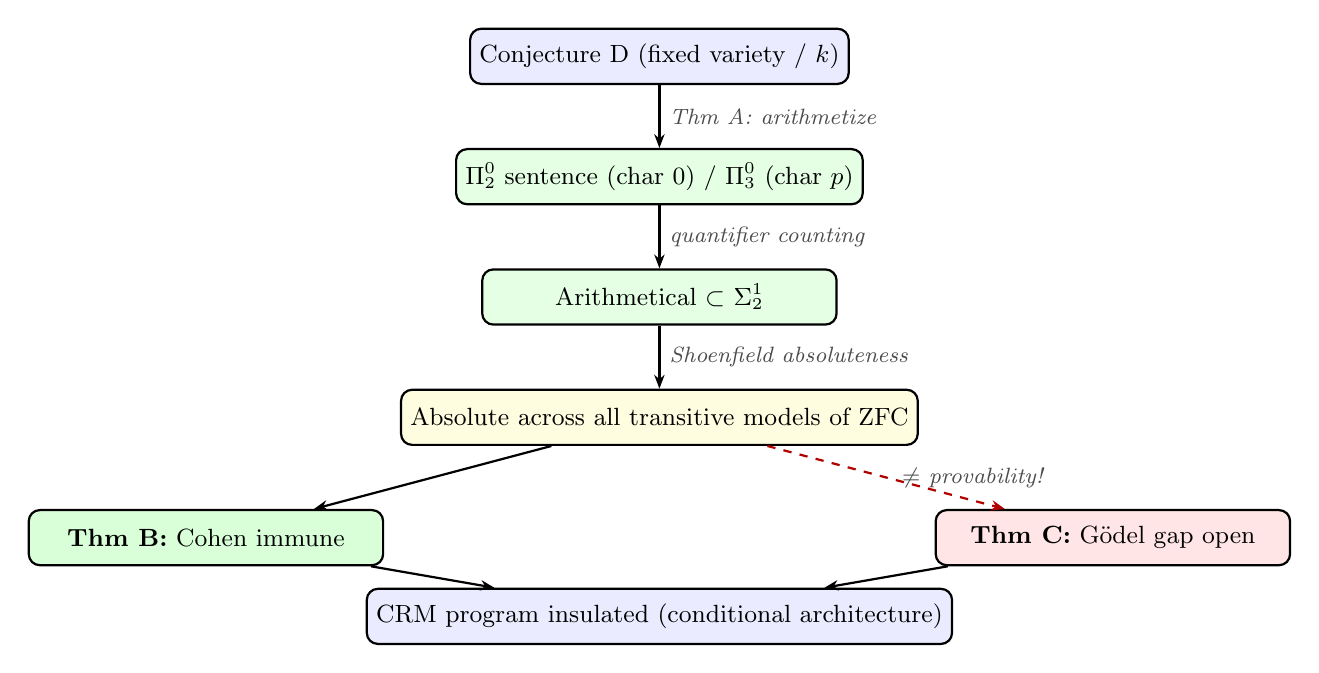
\begin{tikzpicture}[
  box/.style={draw, rounded corners=4pt, thick, minimum width=4.5cm,
              minimum height=0.7cm, align=center, font=\small},
  arr/.style={-{Stealth[length=5pt]}, thick},
  darr/.style={-{Stealth[length=5pt]}, thick, dashed, red!70!black},
  note/.style={font=\footnotesize\itshape, text=gray!60!black}
]
  % Top: Conjecture D
  \node[box, fill=blue!8] (conjd) {Conjecture D (fixed variety / $k$)};

  % Theorem A
  \node[box, fill=green!10, below=0.8cm of conjd] (pi02)
    {$\Pi^0_2$ sentence (char $0$) / $\Pi^0_3$ (char $p$)};
  \draw[arr] (conjd) -- node[right, note] {Thm A: arithmetize} (pi02);

  % Containment
  \node[box, fill=green!10, below=0.8cm of pi02] (arith)
    {Arithmetical $\subset$ $\Sigma^1_2$};
  \draw[arr] (pi02) -- node[right, note] {quantifier counting} (arith);

  % Shoenfield
  \node[box, fill=yellow!12, below=0.8cm of arith] (abs)
    {Absolute across all transitive models of $\ZFC$};
  \draw[arr] (arith) -- node[right, note] {Shoenfield absoluteness} (abs);

  % Branch: Cohen immune
  \node[box, fill=green!15, below left=0.8cm and 0.2cm of abs] (cohen)
    {\textbf{Thm B:} Cohen immune};
  \draw[arr] (abs) -- (cohen);

  % Branch: Gödel gap
  \node[box, fill=red!10, below right=0.8cm and 0.2cm of abs] (goedel)
    {\textbf{Thm C:} G\"odel gap open};
  \draw[darr] (abs) -- node[right, note, xshift=2pt] {$\neq$ provability!} (goedel);

  % CRM insulation
  \node[box, fill=blue!8, below=1.8cm of abs] (crm)
    {CRM program insulated (conditional architecture)};
  \draw[arr] (cohen)  -- (crm);
  \draw[arr] (goedel) -- (crm);
\end{tikzpicture}
\caption{The logical chain of the paper.  Solid arrows are proved implications;
the dashed arrow marks the gap between absoluteness and provability.
The CRM program is insulated from both outcomes by its conditional
(DPT axioms $\Rightarrow$ conclusion) architecture.}
\label{fig:chain}
\end{figure}

\noindent We retain the ``Theorem'' labels for consistency with the Lean formalization, which verifies the logical implications as formal theorems.  The reader should understand that A~follows from standard computability of algebraic geometry plus Grothendieck's spreading-out, B~is an immediate corollary of~A plus Shoenfield, and C~is a standard observation about $\Con(\ZFC)$.  The novelty lies in bringing these together and drawing out the consequences for the CRM program.

\subsection{Constructive Reverse Mathematics: a brief primer}

$\CRM$ calibrates mathematical statements against logical principles of increasing strength within Bishop-style constructive mathematics ($\BISH$).  The principal omniscience principles are:
\begin{itemize}[nosep]
\item $\LPO$ (Limited Principle of Omniscience): every binary sequence is identically zero or contains a~$1$.
\item $\WLPO$ (Weak LPO): every binary sequence is identically zero or is not identically zero, without locating the~$1$.
\item $\MP$ (Markov's Principle): a binary sequence that is not identically zero contains a~$1$.
\end{itemize}
Over $\BISH$, we have $\LPO \Rightarrow \WLPO$ and $\LPO \Rightarrow \MP$, but $\WLPO$ and $\MP$ are in general \emph{incomparable}: neither implies the other over~$\BISH$.  Together they recover~$\LPO$: $\BISH + \WLPO + \MP = \BISH + \LPO$.  The CRM program therefore tracks which of these principles a theorem requires, rather than placing all theorems on a single linear chain.  For a thorough treatment of $\CRM$, see Bridges--Richman~\cite{BridgesRichman1987}; for the broader program of which this paper is part, see Paper~54~\cite{Paper54}.

\subsection{Current state of the art}

Three research programs have approached the logical status of algebraic geometry conjectures from different angles, forming the landscape in which this paper sits.

\textbf{Macintyre~\cite{Macintyre2003}} showed that the notion of a Weil cohomology theory is \emph{first-order} in the model-theoretic sense, implying that the Standard Conjectures encode arithmetical uniformities.  This is the closest precursor to our~$\Pi^0_2$ observation: if Weil cohomology is first-order, then statements about algebraic cycles within a fixed cohomology theory are arithmetical.  However, Macintyre's interest was the decidability of theories and the uniformity of zeta function computations, not the independence of individual conjectures from~$\ZFC$.

\textbf{McLarty~\cite{McLarty2010,McLarty2020}} asked whether Grothendieck's cohomological machinery, which uses universes (equivalent to large cardinal axioms), requires that logical strength.  His answer was no: finite-order arithmetic suffices for the proofs of Fermat's Last Theorem and, more generally, for the cohomology of schemes.  This confirms that algebraic geometry lives in the arithmetical world---consistent with our observation that Conjecture~D is~$\Pi^0_2$---but McLarty asked about proof-theoretic \emph{reduction}, not \emph{independence}.

\textbf{Friedman~\cite{Friedman1999}} conjectured in~1999 that every theorem published in the \emph{Annals of Mathematics} whose statement is arithmetical can be proved in~$\EFA$ (Elementary Function Arithmetic), a system weaker than~$\PA$.  If the Grand Conjecture applies to Conjecture~D, G\"odel independence is ruled out entirely.  Evidence includes Avigad's demonstration~\cite{Avigad2003} that significant number-theoretic results are provable in~$\EFA$.  However, natural counterexamples exist (the graph minor theorem, Friedman's own Boolean relation theory~\cite{Friedman2001}), and the Grand Conjecture itself is unproved.

\textbf{Zilber~\cite{Zilber2010}} developed the theory of \emph{Zariski geometries}, proving (with Hrushovski) that any one-dimensional ample Zariski geometry is isomorphic to an algebraic curve over an algebraically closed field.  This establishes that algebraic geometry is \emph{logically inevitable}: it is the unique ``rich'' geometry arising from model-theoretic axioms (categoricity, stability).  Zilber calls this \emph{logical perfection}.  Macintyre's first-order characterization of Weil cohomology emerged from this Oxford tradition, and Gavrilovich~\cite{Gavrilovich2018} has explicitly connected Zilber-style categoricity to the Standard Conjectures, conjecturing that model-theoretic uniqueness of \'etale cohomology constrains the motivic Galois group.  Zilber's program provides independent evidence that algebraic geometry is logically tame, but operates at the level of \emph{structures} (categoricity of models) rather than \emph{sentences} (absoluteness of truth values).  The conditional decidability results in Zilber's pseudo-exponentiation program (the complex exponential is decidable \emph{if} Schanuel's conjecture holds) are structurally parallel to our CRM conditional architecture (the motive kills~$\LPO$ \emph{if} the DPT axioms hold).

\textbf{What is new here.}  None of the above programs (i)~explicitly classified Conjecture~D as~$\Pi^0_2$, (ii)~applied Shoenfield absoluteness to rule out Cohen independence, (iii)~distinguished the two modes of independence in the context of algebraic geometry, or (iv)~audited the CRM program's conditional architecture for G\"odel vulnerability.  The synthesis of these steps is the contribution of the present paper.

\subsection{Position in the atlas}

This is Paper~55 of a series applying constructive reverse mathematics across pure mathematics and physics.  Paper~40~\cite{Paper40} established that all physical undecidability is equivalent to~$\LPO$ ($\BISH + \LPO$), with the Cubitt--Perez-Garcia--Wolf spectral gap undecidability~\cite{CubittPW2015} classified as~$\Sigma^0_1$-complete (hence LPO-equivalent).  Paper~26~\cite{Paper26} embedded G\"odel sequences into the bidual gap~$\ell^\infty/c_0$, proving that gap detection is WLPO-complete via an arithmetical calibration chain: $\WLPO \leftrightarrow \Pi^0_1$-consistency decidable $\leftrightarrow$ gap detection decidable.  The present paper addresses the next natural question: does the G\"odel phenomenon---already encountered at $\WLPO$ (Paper~26) and $\LPO$ (Paper~40) in the CRM hierarchy---extend to the meta-level of the motives program?


%% ===================================================================
\section{Preliminaries}
\label{sec:prelim}
%% ===================================================================

\begin{definition}[Arithmetical hierarchy]
\label{def:arith}
A sentence in first-order arithmetic is classified by the pattern of its quantifiers over~$\N$:
\begin{itemize}[nosep]
\item $\Delta^0_0$ (decidable): quantifier-free, or bounded quantifiers only.
\item $\Pi^0_1$: of the form $\forall n \, R(n)$ with $R$ decidable.  Examples: $\Con(\ZFC)$, Goldbach's conjecture.
\item $\Sigma^0_1$: of the form $\exists n \, R(n)$ with $R$ decidable.
\item $\Pi^0_2$: of the form $\forall n \,\exists m \, R(n,m)$ with $R$ decidable.  This is the complexity class of Conjecture~D.
\end{itemize}
Every arithmetical sentence is~$\Sigma^1_2$ and hence within the scope of Shoenfield absoluteness.
\end{definition}

\begin{definition}[Transitive model]
\label{def:transmodel}
A \emph{transitive model} of~$\ZFC$ is a set $M$ that is transitive (if $x \in y \in M$ then $x \in M$) and satisfies all axioms of~$\ZFC$.  Transitive models contain the ``correct'' natural numbers (i.e., the standard~$\N$); this is what makes them relevant for absoluteness.
\end{definition}

\begin{definition}[Absoluteness]
\label{def:absolute}
A sentence~$\varphi$ is \emph{absolute} between transitive models of~$\ZFC$ if every transitive model that satisfies~$\ZFC$ assigns the same truth value to~$\varphi$.  Equivalently, the truth value of~$\varphi$ is invariant under Cohen forcing and the addition of large cardinal axioms.
\end{definition}

\begin{definition}[Two modes of independence]
\label{def:modes}
Let $\varphi$ be a sentence and $T$ a formal system.
\begin{enumerate}
\item \textbf{Cohen independence} (set-theoretic).  $\varphi$ is true in some transitive models of~$T$ and false in others.  This occurs when $\varphi$ is sensitive to the set-theoretic universe (e.g., the Continuum Hypothesis~$\CH$).  \emph{Forcing} is the standard tool for establishing this.

\item \textbf{G\"odel independence} (arithmetical).  $\varphi$ has the same truth value in all transitive models (it is absolute), but $T$ is too weak to prove it.  The truth value is determinate---$\varphi$ is either true-in-all-transitive-models or false-in-all-transitive-models---but $T$'s induction axioms cannot reach it.  The canonical example: $\Con(\ZFC)$ is~$\Pi^0_1$, hence absolute, yet unprovable in~$\ZFC$ by G\"odel's second incompleteness theorem~\cite{Goedel1931}.
\end{enumerate}
\end{definition}

\begin{definition}[Standard Conjecture~D]
\label{def:conjD}
For a smooth projective variety~$X$ over a field~$k$ with Weil cohomology $H^*$, Conjecture~D~\cite{Grothendieck1969} asserts: \emph{numerical equivalence coincides with homological equivalence for algebraic cycles}.  Precisely: if $Z \in Z^r(X)$ satisfies $\deg(Z \cdot W) = 0$ for every test cycle~$W$ of complementary dimension (i.e., $Z \equiv_{\mathrm{num}} 0$), then $\cl(Z) = 0$ in~$H^{2r}(X)$.
\end{definition}

\begin{definition}[Arithmetical encoding of Conjecture~D]
\label{def:encoding}
Let $k$ be a countable algebraically closed field (e.g., $\Qbar$ or~$\overline{\Fq}$) and $X/k$ a smooth projective variety.  Since $k$ admits an algorithmic presentation, the following objects are effectively enumerable:
\begin{enumerate}[nosep]
\item Algebraic cycles $Z \in \Zr(X)$: each defined by a finite ideal of polynomials in~$k[x_0, \ldots, x_n]$.
\item Test cycles $W$: likewise enumerable.
\item Intersection numbers $\deg(Z \cdot W) \in \Z$: computable by Gr\"obner basis methods.
\item The cycle class $\cl(Z) \in H^{2r}_{\mathrm{dR}}(X/k)$: in characteristic~$0$, computable by algorithms in $D$-module theory~\cite{OakuTakayama1999}; in positive characteristic, computable modulo~$\ell^c$ for any precision~$c$ via $\ell$-adic or crystalline methods (see Theorem~\ref{thm:A}, Step~4).
\end{enumerate}
\end{definition}

\begin{definition}[DPT axioms]
\label{def:dpt}
The DPT axioms (Papers~51--53~\cite{Paper51}) are the hypotheses under which the CRM program's motive kills~$\LPO$:
\begin{enumerate}[nosep]
\item \emph{Decidable equality} on algebraic cycles.
\item \emph{Algebraic spectrum}: eigenvalues of Frobenius are algebraic numbers.  (Classically, this is a theorem of Deligne~(Weil~II, 1980); the CRM program treats it as a hypothesis because Deligne's proof uses excluded middle.)
\item \emph{Archimedean polarization}: positive-definiteness of the N\'eron-Tate height.
\end{enumerate}
These are first-order algebraic properties, verifiable case by case, and the CRM conditional takes the form: DPT axioms $\Rightarrow$ motive reduces~$\LPO$ to~$\MP$.
\end{definition}


%% ===================================================================
\section{Main Results}
\label{sec:results}
%% ===================================================================

\subsection{Theorem A: $\Pi^0_2$ Classification}

\begin{theorem}[Theorem A: arithmetical classification for a fixed variety]
\label{thm:A}
Standard Conjecture~D for a fixed smooth projective variety~$X$ over a countable algebraically closed field~$k$ is an arithmetical sentence.  In characteristic~$0$, it is~$\Pi^0_2$.  In positive characteristic, cycle class vanishing degrades to a~$\Pi^0_1$ predicate (over the $\ell$-adic precision parameter), making the full statement~$\Pi^0_3$.  In either case, the sentence is within the scope of Shoenfield absoluteness.
\end{theorem}

\begin{proof}
We proceed in four steps: state the conjecture, rewrite it in prenex form, verify that the quantifiers range over~$\N$, and verify that the matrix is decidable.

\medskip\noindent
\textbf{Step 1: Statement.}  Fix a smooth projective variety~$X$ of dimension~$d$ over a countable algebraically closed field~$k$, and fix a Weil cohomology theory $H^*$ (e.g., algebraic de Rham cohomology when $\mathrm{char}(k) = 0$, or $\ell$-adic cohomology when $\mathrm{char}(k) = p > 0$).  For each integer $0 \leq r \leq d$, the cycle class map sends an algebraic cycle $Z \in Z^r(X)$ to a cohomology class $\cl(Z) \in H^{2r}(X)$.  Conjecture~D for~$X$ asserts:
\[
  \forall Z \in \Zr(X),\quad Z \equiv_{\mathrm{num}} 0 \;\;\Longrightarrow\;\; \cl(Z) = 0.
\]
Expanding the definition of numerical equivalence, this reads:
\begin{equation}\label{eq:conjD-expanded}
  \forall Z \in \Zr(X) \;\Big[ \big(\forall W \in Z^{d-r}(X),\; \deg(Z \cdot W) = 0\big) \;\Longrightarrow\; \cl(Z) = 0 \Big].
\end{equation}

\medskip\noindent
\textbf{Step 2: Prenex normal form.}  The implication $P \Rightarrow Q$ is classically equivalent to $\lnot P \lor Q$.  Applying this to~\eqref{eq:conjD-expanded} and pushing the negation through the inner universal quantifier (note: this step uses classical logic, specifically $\lnot\forall \equiv \exists\lnot$; however, this is strictly a meta-level syntactic reduction to classify the sentence within the classical arithmetical hierarchy for the purpose of applying Shoenfield's theorem---it does not introduce classical logic into the internal $\BISH$ calibrations of the CRM program):
\begin{align*}
&\forall Z \;\Big[ \big(\exists W,\; \deg(Z \cdot W) \neq 0\big) \;\lor\; \cl(Z) = 0 \Big] \\
\equiv\quad &\forall Z \;\exists W \;\Big[ \deg(Z \cdot W) \neq 0 \;\lor\; \cl(Z) = 0 \Big].
\end{align*}
The second line follows because if $\cl(Z) = 0$, the existential is trivially witnessed by any~$W$ (the disjunction holds via the second disjunct); and if $\cl(Z) \neq 0$ but $Z \equiv_{\mathrm{num}} 0$ fails, there exists a specific~$W$ witnessing $\deg(Z \cdot W) \neq 0$.  The result is a sentence in \emph{prenex} $\forall\exists$ form.

\medskip\noindent
\textbf{Step 3: Arithmetization of quantifiers.}  Since $k$ is countable and admits an algorithmic presentation (e.g., $\Qbar$ via minimal polynomials over~$\Q$, or $\overline{\Fq}$ via irreducible polynomials over~$\Fq$), every algebraic cycle $Z \in Z^r(X)$ is a finite formal $\Z$-linear combination of subvarieties, each defined by finitely many polynomial equations with coefficients in~$k$.  This data can be G\"odel-numbered: there is a computable bijection between algebraic cycles (of all codimensions, on~$X$) and a subset of~$\N$.

Concretely, a cycle $Z = \sum_{i=1}^s n_i [V_i]$ is encoded by the tuple $(r, s, n_1, \ldots, n_s, \text{code}(V_1), \ldots, \text{code}(V_s))$, where $\text{code}(V_i)$ is a G\"odel number for the defining ideal of~$V_i$ in $k[x_0, \ldots, x_n]$ (the ambient projective space being part of the fixed data of~$X$).  Similarly, test cycles~$W$ are enumerable.  The quantifiers $\forall Z$ and $\exists W$ both range over~$\N$.

\medskip\noindent
\textbf{Step 4: Decidability of the matrix.}  Define $R(n, m) \;:=\; [\deg(Z_n \cdot W_m) \neq 0 \;\lor\; \cl(Z_n) = 0]$, where $Z_n$ is the cycle with G\"odel number~$n$ and $W_m$ the test cycle with G\"odel number~$m$.  We must show $R$ is a decidable (i.e., computable) predicate.

\begin{itemize}
\item \textbf{Intersection numbers are computable.}  Given $Z_n$ and $W_m$, the intersection product $Z_n \cdot W_m$ is a zero-cycle on~$X$.  Its degree $\deg(Z_n \cdot W_m) \in \Z$ is computable by Gr\"obner basis algorithms: one computes the intersection scheme (via ideal operations in $k[x_0, \ldots, x_n]$), then reads off the degree as a sum of local multiplicities, each of which is the length of a local Artinian ring (computable by standard commutative algebra).  In particular, the predicate $\deg(Z_n \cdot W_m) \neq 0$ is decidable.

\item \textbf{Cycle class vanishing is computable.}  In characteristic~$0$, the cycle class $\cl(Z_n) \in H^{2r}_{\mathrm{dR}}(X/k)$ is a vector in a \emph{finite-dimensional} $k$-vector space.  Oaku--Takayama~\cite{OakuTakayama1999} gave an algorithm for computing de Rham cohomology groups (and cycle classes therein) via $D$-module theory.  Given the finite-dimensional presentation of $H^{2r}_{\mathrm{dR}}(X/k)$, the predicate $\cl(Z_n) = 0$ reduces to checking whether a vector in a finite-dimensional space is the zero vector, which is decidable by comparing finitely many coordinates in the decidable field~$k$.

In positive characteristic ($k = \overline{\F_q}$), Weil cohomology takes values in $\ell$-adic or crystalline coefficient fields ($\Qell$ or $W(k) \otimes \Q$).  The Betti numbers $\dim H^{2r}(X)$ and the characteristic polynomial of Frobenius are computable by the algorithms of Kedlaya and Lauder (via rigid or $p$-adic cohomology).  However, these algorithms compute \emph{traces of Frobenius} (zeta function data), not individual cycle classes.  Computing $\cl(Z_n) \in H^{2r}_{\ell\text{-adic}}(X)$ for a specific algebraic cycle~$Z_n$ requires $\ell$-adic computations: one can evaluate $\cl(Z_n) \bmod \ell^c$ for any given precision~$c$, and $\cl(Z_n) = 0$ iff $\cl(Z_n) \equiv 0 \pmod{\ell^c}$ for all~$c$.  This makes the predicate ``$\cl(Z_n) = 0$'' a $\Pi^0_1$ statement (over the precision parameter~$c$), and the full conjecture degrades to~$\Pi^0_3$ in positive characteristic.  This is still strictly arithmetical and well within the scope of Shoenfield absoluteness; the classification as ``absolute and Cohen-immune'' is unaffected.
\end{itemize}

In characteristic~$0$, both disjuncts are decidable, so $R(n,m)$ is decidable.  The sentence $\forall n \,\exists m \, R(n,m)$ has the canonical $\Pi^0_2$ form: a universal quantifier over~$\N$, followed by an existential quantifier over~$\N$, applied to a decidable relation (Figure~\ref{fig:pipeline}).  In positive characteristic, $R(n,m)$ is~$\Pi^0_1$ (due to the $\ell$-adic precision parameter), making the full sentence~$\Pi^0_3$.
\end{proof}

\begin{figure}[ht]
\centering
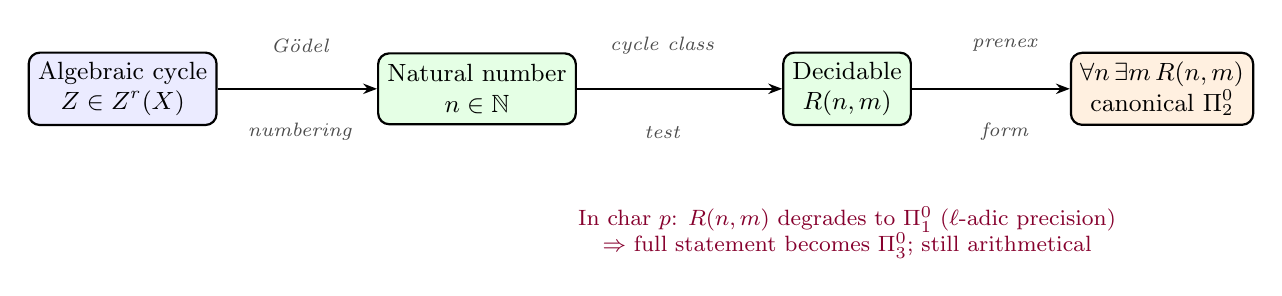
\begin{tikzpicture}[
  box/.style={draw, rounded corners=4pt, thick,
              minimum height=0.9cm, align=center, font=\small},
  arr/.style={-{Stealth[length=5pt]}, thick},
  note/.style={font=\scriptsize\itshape, text=gray!60!black},
  annot/.style={font=\footnotesize, text=purple!70!black, align=center}
]
  % Row 1: boxes — spread out to give labels room
  \node[box, fill=blue!8] (cycle) at (0,0) {Algebraic cycle\\$Z \in Z^r(X)$};
  \node[box, fill=green!10] (nat) at (4.5,0) {Natural number\\$n \in \N$};
  \node[box, fill=green!10] (pred) at (9.2,0) {Decidable\\$R(n,m)$};
  \node[box, fill=orange!12] (pi02) at (13.2,0) {$\forall n\,\exists m\, R(n,m)$\\canonical $\Pi^0_2$};

  % Arrows with labels placed well above/below the line
  \draw[arr] (cycle) -- (nat);
  \node[note] at (2.25,0.55) {G\"odel};
  \node[note] at (2.25,-0.55) {numbering};

  \draw[arr] (nat) -- (pred);
  \node[note] at (6.85,0.55) {cycle class};
  \node[note] at (6.85,-0.55) {test};

  \draw[arr] (pred) -- (pi02);
  \node[note] at (11.2,0.55) {prenex};
  \node[note] at (11.2,-0.55) {form};

  % Annotation for char p degradation
  \node[annot, below=0.9cm of pred]
    {In char $p$: $R(n,m)$ degrades to $\Pi^0_1$ ($\ell$-adic precision)\\
     $\Rightarrow$ full statement becomes $\Pi^0_3$; still arithmetical};
\end{tikzpicture}
\caption{The arithmetization pipeline for Standard Conjecture~D (characteristic~$0$).
Each step preserves decidability of the base predicates; the prenex form reveals the~$\Pi^0_2$ classification.
In positive characteristic, the cycle class test acquires an extra quantifier (over $\ell$-adic precision).}
\label{fig:pipeline}
\end{figure}


\begin{theorem}[Theorem A, global version]
\label{thm:A-global}
Global Conjecture~D (quantifying over all smooth projective varieties over all algebraically closed fields) is equivalent to Conjecture~D for all smooth projective varieties over~$\Qbar$ (in characteristic~$0$) and over~$\overline{\Fq}$ for all primes~$q$ (in positive characteristic).  The characteristic-$0$ component is~$\Pi^0_2$; the positive-characteristic component is~$\Pi^0_3$; the conjunction is~$\Pi^0_3$.  In all cases, the statement is arithmetical and within the scope of Shoenfield absoluteness.
\end{theorem}

\begin{proof}
The global conjecture quantifies over all smooth projective varieties~$X$ over all algebraically closed fields~$K$---a priori, this is a quantifier over a proper class.  We reduce it to a countable quantification in three steps.

\medskip\noindent
\textbf{Step 1: Spreading out (characteristic $0$)~\cite{Grothendieck1969}.}  Let $K$ be an uncountable algebraically closed field of characteristic~$0$ (e.g., $K = \C$), and let $X/K$ be a smooth projective variety.  The defining equations of~$X$ involve finitely many elements of~$K$.  These elements generate a finitely generated extension $F = \Q(\alpha_1, \ldots, \alpha_s) \subset K$.  By EGA~IV, $X$ is defined over~$F$: there exists a smooth projective variety $X_F / F$ with $X \cong X_F \times_F K$.

Note that $F$ may have positive transcendence degree over~$\Q$ (e.g., if some~$\alpha_i$ is transcendental), so $F$ need not embed into~$\Qbar$.  Instead, we spread out $X_F$ to a smooth proper family $\mathcal{X} \to S$ over a base scheme $S = \mathrm{Spec}(A)$ for some finitely generated $\Q$-algebra~$A$ with fraction field~$F$.  The closed points $s \in S(\Qbar)$ yield smooth projective fibers $X_s$ over residue fields $\kappa(s) \subset \Qbar$.

\emph{Preservation of the conjecture.}  Conjecture~D asserts that numerical equivalence coincides with homological equivalence, i.e., $\ker(\cl) \cap Z^r(X) = \ker(\mathrm{num}) \cap Z^r(X)$.  Equivalently, the cycle class map $\cl \colon \mathrm{CH}^r(X)_{\mathrm{num}} \otimes \Q \to H^{2r}(X)$ is \emph{injective}.  (Note: the intersection pairing on $\mathrm{CH}^r_{\mathrm{num}} \otimes \Q$ is non-degenerate \emph{by definition}---numerical equivalence quotients out the kernel---so non-degeneracy of the pairing is not the content of Conjecture~D.  The content is that every cycle killed by intersection numbers is also killed by the cycle class map.)

Suppose $D(X/K)$ holds.  We must show $D(X_s / \kappa(s))$ holds for some closed point $s \in S(\Qbar)$.  A na\"ive specialization of cycles is delicate: the fiber~$X_s$ may acquire algebraic cycles not liftable to the generic fiber (Chow rank jumping).  However, the \emph{contrapositive} is clean.  If $D$ fails over~$\Qbar$---i.e., there exists a variety $Y/\Qbar$ and a cycle $Z \in Z^r(Y)$ with $Z \equiv_{\mathrm{num}} 0$ but $\cl(Z) \neq 0$---then $Y$ and $Z$ are defined over a finitely generated extension of~$\Q$, and by base change to any algebraically closed field containing that extension, the counterexample persists (cycle classes and intersection numbers are preserved by flat base change of algebraically closed fields).  Hence $D$ fails over~$K$.  Contrapositively, $D(K) \Rightarrow D(\Qbar)$.

\medskip\noindent
\textbf{Step 2: Lefschetz principle~\cite{Kleiman1968}.}  For two algebraically closed fields $k_1 \subset k_2$ of the same characteristic, the functor $X \mapsto X \times_{k_1} k_2$ is faithful on algebraic cycles and preserves intersection numbers and cycle classes.  In characteristic~$0$, every algebraically closed field contains~$\Qbar$, so any counterexample to Conjecture~D over any algebraically closed field of characteristic~$0$ descends to a counterexample over~$\Qbar$ by Step~1.  In characteristic~$p > 0$, any algebraically closed field contains~$\overline{\Fq}$ for some prime power~$q$, and the same argument applies.

\medskip\noindent
\textbf{Step 3: Countable reduction.}  Steps~1 and~2 show that global Conjecture~D is equivalent to:
\[
  \bigwedge_{p \text{ prime or } 0} \;\forall X / k_p,\quad D(X)
\]
where $k_0 = \Qbar$ and $k_p = \overline{\F_p}$ for primes~$p$.  Each field~$k_p$ is countable.  The set of isomorphism classes of smooth projective varieties over a countable field is countable (parameterized by finitely many polynomial equations with coefficients in the countable field).  So the quantifier ``$\forall X / k_p$'' ranges over a countable set, which we enumerate as~$\N$.

The full global conjecture then takes the form:
\[
  \forall p \;\forall i \;\forall n \;\exists m \; R_p(i, n, m)
\]
where $p$ ranges over primes and~$0$ (countable), $i$ enumerates varieties over~$k_p$, $n$ encodes cycles, and $m$ encodes test cycles.  Absorbing the three universal quantifiers into a single~$\forall$ (via a pairing function $\N^3 \to \N$) yields a sentence of the form $\forall N \,\exists m \, R'(N, m)$ when restricted to characteristic~$0$ (where $R'$ is decidable, giving~$\Pi^0_2$).  For the full global conjecture including positive characteristic, $R'$ is~$\Pi^0_1$ (due to the $\ell$-adic precision parameter), so the conjunction is~$\Pi^0_3$---still strictly arithmetical.
\end{proof}


\subsection{Theorem B: Cohen Immunity}

We first recall the key external theorem, then apply it to Conjecture~D.

\begin{theorem}[Shoenfield, 1961~\cite{Shoenfield1961}]
\label{thm:shoenfield}
Let $V$ be a model of~$\ZFC$ and let $V[G]$ be a generic extension obtained by Cohen forcing.  Then for every $\Sigma^1_2$ sentence~$\varphi$ (and hence for every arithmetical sentence):
\[
  V \models \varphi \quad\Longleftrightarrow\quad V[G] \models \varphi.
\]
More generally, every $\Sigma^1_2$ sentence is absolute between any two transitive models of~$\ZFC$ that contain the same ordinals.\footnote{The ``same ordinals'' clause is needed for~$\Sigma^1_2$ sentences involving quantification over sets of natural numbers.  For purely arithmetical sentences (including~$\Pi^0_2$), the clause is vacuous: such sentences depend only on~$\N$, which is the same in all transitive models.}
\end{theorem}

The logical chain is: $\Pi^0_2 \subset \text{arithmetical} \subset \Sigma^1_2 \subset \text{scope of Shoenfield}$.  The containment $\Pi^0_2 \subset \text{arithmetical}$ holds because $\Pi^0_2$ sentences quantify only over~$\N$ with a decidable matrix.  The containment arithmetical $\subset \Sigma^1_2$ holds because arithmetical sentences involve only number quantifiers, while $\Sigma^1_2$ allows a block of set quantifiers followed by number quantifiers.

\begin{theorem}[Theorem B: Cohen immunity of Conjecture~D]
\label{thm:B}
Standard Conjecture~D cannot be made true or false by Cohen forcing.  Its truth value is the same in all transitive models of~$\ZFC$.  In particular:
\begin{enumerate}[nosep]
\item The Continuum Hypothesis ($\CH$) is irrelevant to Conjecture~D.
\item Martin's Axiom is irrelevant to Conjecture~D.
\item Large cardinal axioms do not change the truth value of Conjecture~D.\footnote{Large cardinals can change which sentences are \emph{provable} from $\ZFC$ + large cardinals, but cannot change the truth value of arithmetical sentences in transitive models.}
\end{enumerate}
No ``non-standard variety'' can be forced into existence that violates~D while all standard varieties satisfy it.
\end{theorem}

\begin{proof}
We give a detailed proof by chaining the classification and absoluteness results.

\medskip\noindent
\textbf{Step 1: Classification.}  By Theorem~\ref{thm:A}, Conjecture~D is arithmetical: $\Pi^0_2$ in characteristic~$0$, $\Pi^0_3$ in positive characteristic.  By Theorem~\ref{thm:A-global}, the global version is~$\Pi^0_3$.  In all cases, the sentence is arithmetical and hence~$\Sigma^1_2$.

\medskip\noindent
\textbf{Step 2: Containment in~$\Sigma^1_2$.}  Every $\Pi^0_2$ sentence is arithmetical (its quantifiers range only over~$\N$).  Every arithmetical sentence is $\Sigma^1_2$: informally, an arithmetical sentence uses no set quantifiers, while $\Sigma^1_2$ allows $\exists X \subseteq \N \,\forall Y \subseteq \N \,\theta(X,Y)$ where $\theta$ is arithmetical---simply take the set quantifiers to be vacuous.  Hence $D$ is within the scope of Shoenfield's theorem.

\medskip\noindent
\textbf{Step 3: Application of absoluteness.}  Let $V$ be any transitive model of~$\ZFC$, and let $V[G]$ be any generic extension by forcing.  By Theorem~\ref{thm:shoenfield}:
\[
  V \models D \quad\Longleftrightarrow\quad V[G] \models D.
\]
This means that no forcing construction can change the truth value of~$D$.

\medskip\noindent
\textbf{Step 4: Specific consequences.}  The Continuum Hypothesis ($\CH$) is proved consistent with~$\ZFC$ by G\"odel's constructible universe~$L$, and proved independent by Cohen forcing.  But since $D$ has the same truth value in~$V$ and in any $V[G]$ obtained by forcing, neither adding~$\CH$ nor adding~$\lnot\CH$ by forcing changes~$D$'s truth value.  The same argument applies to Martin's Axiom (established by iterated forcing) and to any statement whose independence is witnessed by forcing.

For large cardinals: if $\kappa$ is a large cardinal in~$V$, the inner model $L[U]$ (for a measurable cardinal) or the extension $V[G]$ (for forcing with a large cardinal) both satisfy the same arithmetical sentences as~$V$.  Hence large cardinals do not affect~$D$.

\medskip\noindent
\textbf{Step 5: No ``non-standard counterexamples.''}  One might worry: could a forcing extension $V[G]$ contain a ``new'' smooth projective variety that violates~$D$?  No.  The varieties over~$\Qbar$ are determined by polynomial equations with coefficients in~$\Qbar$, and $\Qbar$ is absolute between transitive models (it is the unique algebraic closure of~$\Q$, which is definable in any model containing~$\N$).  No new varieties over~$\Qbar$ appear in~$V[G]$; and the truth of~$D$ for each variety is an arithmetical statement, hence absolute.
\end{proof}

\begin{corollary}
\label{cor:ch-irrelevant}
Assuming Conjecture~D is true (in the standard model), it is true in every transitive model of~$\ZFC + \CH$, every transitive model of~$\ZFC + \lnot\CH$, every transitive model of~$\ZFC +$~Martin's Axiom, and every transitive model of~$\ZFC +$~(large cardinal axiom).  Conversely, if Conjecture~D is false, it is false in all of these.
\end{corollary}


\subsection{Theorem C: The G\"odel Gap}

The crucial point of this subsection is that the immunity established by Theorem~B eliminates only \emph{one} of two distinct modes of independence (Figure~\ref{fig:modes}).  We now develop the second mode carefully.

\begin{observation}[Absoluteness $\neq$ Provability: the $\Con(\ZFC)$ witness]
\label{obs:gap}
The sentence $\Con(\ZFC)$ is defined as: ``there is no natural number~$n$ that encodes a proof of~$0 = 1$ from the axioms of~$\ZFC$.''  Formally:
\[
  \Con(\ZFC) \;:=\; \forall n \in \N,\; \lnot\mathrm{Proof}_{\ZFC}(n, \ulcorner 0 = 1 \urcorner).
\]
This is a $\Pi^0_1$ sentence: a single universal quantifier over~$\N$ applied to a decidable predicate (``$n$ does not encode a valid proof of~$0=1$'' is decidable---one can mechanically check whether a finite string is a valid proof).

Since $\Pi^0_1 \subset \Pi^0_2 \subset \Sigma^1_2$, Shoenfield's theorem applies: $\Con(\ZFC)$ is absolute across all transitive models.  In every transitive model of~$\ZFC$, the natural numbers are standard (i.e., they are the genuine~$\N$), so $\Con(\ZFC)$ has the same truth value everywhere.

Yet G\"odel's Second Incompleteness Theorem~\cite{Goedel1931} establishes:
\[
  \ZFC \nvdash \Con(\ZFC) \qquad\text{(assuming $\ZFC$ is consistent)}.
\]
Moreover, soundness of~$\ZFC$ implies $\ZFC \nvdash \lnot\Con(\ZFC)$ (if $\ZFC$ is consistent, it cannot prove its own inconsistency without being inconsistent).  So $\Con(\ZFC)$ is \emph{independent} of~$\ZFC$---but not in the Cohen sense.  It is absolute (same truth value in all transitive models), yet unprovable.  This is G\"odel independence.
\end{observation}

\begin{definition}[Two modes of independence, revisited]
\label{def:modes-revisited}
The $\Con(\ZFC)$ example motivates a sharp distinction:
\begin{enumerate}
\item \textbf{Cohen independence.}  A sentence~$\varphi$ is Cohen-independent of~$\ZFC$ if there exist transitive models $M_1, M_2 \models \ZFC$ with $M_1 \models \varphi$ and $M_2 \models \lnot\varphi$.  Equivalently, both $\ZFC + \varphi$ and $\ZFC + \lnot\varphi$ have transitive models.  The Continuum Hypothesis is the paradigmatic example.

\emph{Mechanism:} Forcing constructs a new transitive model $V[G]$ from an old one~$V$ by adjoining a ``generic'' set~$G$.  The new model may satisfy different sentences from the old one---but only sentences above the $\Sigma^1_2$ threshold.  Arithmetical sentences are immune.

\item \textbf{G\"odel independence.}  A sentence~$\varphi$ is G\"odel-independent of~$\ZFC$ if (a)~$\varphi$ is absolute (same truth value in all transitive models) but (b)~$\ZFC$ can prove neither~$\varphi$ nor~$\lnot\varphi$.  The truth value is determined---$\varphi$ is either ``true everywhere'' or ``false everywhere''---but $\ZFC$'s deductive apparatus cannot reach it.

\emph{Mechanism:} The sentence is too ``deep'' arithmetically for~$\ZFC$'s induction axioms to establish.  The proof would require stronger induction principles (e.g., those available in $\ZFC +$ ``there exists an inaccessible cardinal,'' or in second-order arithmetic with stronger comprehension).  Non-transitive models (which contain ``non-standard'' natural numbers) may disagree with the standard truth value, but these models are pathological from the standpoint of arithmetic.
\end{enumerate}
\end{definition}

\begin{theorem}[Theorem C: G\"odel gap for Conjecture~D]
\label{thm:C}
Standard Conjecture~D satisfies:
\begin{enumerate}
\item \textbf{Cohen independence is impossible.}  Conjecture~D has the same truth value in every transitive model of~$\ZFC$.
\item \textbf{G\"odel independence is not ruled out.}  It remains logically possible that Conjecture~D is true (in all transitive models) but unprovable in~$\ZFC$.
\item \textbf{The two modes are mutually exclusive.}  No sentence can be both Cohen-independent and G\"odel-independent of~$\ZFC$.
\end{enumerate}
\end{theorem}

\begin{proof}
\textbf{Part (1).}  This is Theorem~\ref{thm:B}.  Conjecture~D is arithmetical ($\Pi^0_2$ in characteristic~$0$, $\Pi^0_3$ in positive characteristic; Theorem~\ref{thm:A}), hence $\Sigma^1_2$, hence absolute by Shoenfield's theorem.  Therefore it has the same truth value in all transitive models.  In particular, there cannot exist transitive models $M_1 \models D$ and $M_2 \models \lnot D$---the defining condition of Cohen independence fails.

\medskip\noindent
\textbf{Part (2).}  We argue by analogy with $\Con(\ZFC)$ and then explain why no known metatheorem closes the gap.

The sentence $\Con(\ZFC)$ demonstrates that the following situation is logically consistent:
\begin{quote}
A sentence~$\varphi$ is absolute across all transitive models of~$\ZFC$ (so its truth value is determined), yet $\ZFC$ cannot prove~$\varphi$.
\end{quote}
Conjecture~D is in the same broad family (arithmetical, at $\Pi^0_2$ or~$\Pi^0_3$ depending on characteristic---in any case at higher complexity than $\Con(\ZFC)$, which is merely~$\Pi^0_1$).  To rule out G\"odel independence for~$D$, one would need one of:
\begin{itemize}[nosep]
\item A proof of~$D$ in~$\ZFC$ (i.e., resolving the conjecture positively---an open problem in algebraic geometry).
\item A refutation of~$D$ in~$\ZFC$ (i.e., a counterexample variety---no evidence for this).
\item A metatheorem of the form: ``every true~$\Pi^0_2$ sentence of complexity at most $C$ is provable in~$\ZFC$'' where $C$ bounds the complexity of~$D$.  No such metatheorem is known.
\end{itemize}
The statement ``$\ZFC$ proves Conjecture~D'' is itself a~$\Sigma^0_1$ sentence (``there exists a proof''), and we have no proof of this~$\Sigma^0_1$ sentence.  So the G\"odel-independence scenario remains open.

\medskip\noindent
\textbf{Part (3).}  This is immediate from the definitions but worth stating explicitly to complete the trichotomy.  Suppose for contradiction that a sentence~$\varphi$ is both Cohen-independent and G\"odel-independent of~$\ZFC$.

Cohen independence means: there exist transitive models $M_1 \models \varphi$ and $M_2 \models \lnot\varphi$.

G\"odel independence means, by Definition~\ref{def:modes-revisited}(2): $\varphi$ is \emph{absolute}---it has the same truth value in all transitive models.

But if $\varphi$ is absolute, then $M_1 \models \varphi \Leftrightarrow M_2 \models \varphi$, contradicting $M_1 \models \varphi$ and $M_2 \models \lnot\varphi$.  So the two modes are mutually exclusive: a sentence can be at most one of Cohen-independent or G\"odel-independent (or neither, if it is both absolute and provable---e.g., ``$2 + 2 = 4$'').
\end{proof}

\begin{figure}[ht]
\centering
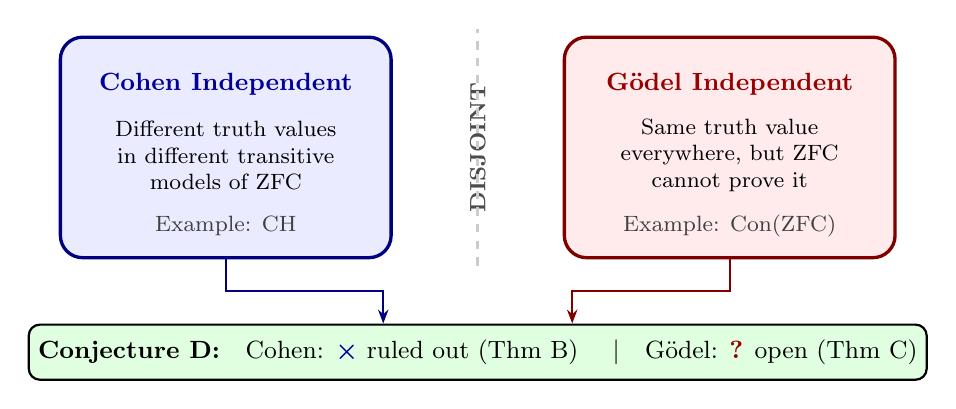
\begin{tikzpicture}[
  region/.style={draw, very thick, rounded corners=8pt, minimum width=4.2cm,
                 minimum height=2.8cm, align=center},
  ex/.style={font=\footnotesize, text=gray!50!black},
  arr/.style={-{Stealth[length=5pt]}, thick}
]
  % Cohen region (left)
  \node[region, fill=blue!8, draw=blue!50!black] (cohen) at (-3.2,0) {};
  \node[font=\small\bfseries, text=blue!60!black] at (-3.2,0.8) {Cohen Independent};
  \node[font=\footnotesize, align=center, text width=3.6cm] at (-3.2,-0.1)
    {Different truth values\\in different transitive\\models of $\ZFC$};
  \node[ex] at (-3.2,-1.0) {Example: $\CH$};

  % Gödel region (right)
  \node[region, fill=red!8, draw=red!50!black] (goedel) at (3.2,0) {};
  \node[font=\small\bfseries, text=red!60!black] at (3.2,0.8) {G\"odel Independent};
  \node[font=\footnotesize, align=center, text width=3.6cm] at (3.2,-0.1)
    {Same truth value\\everywhere, but $\ZFC$\\cannot prove it};
  \node[ex] at (3.2,-1.0) {Example: $\Con(\ZFC)$};

  % Excluded zone (center gap)
  \node[font=\footnotesize\bfseries, text=gray!60!black, rotate=90] at (0,0) {DISJOINT};
  \draw[very thick, gray!40, dashed] (0,-1.5) -- (0,1.5);

  % Conjecture D below
  \node[draw, rounded corners=4pt, thick, fill=green!12, minimum width=6cm,
        minimum height=0.7cm, font=\small, align=center] (conjd) at (0,-2.6)
    {\textbf{Conjecture D:}\quad
     Cohen: \textcolor{blue!60!black}{$\boldsymbol{\times}$} ruled out (Thm B)
     \quad$|$\quad
     G\"odel: \textcolor{red!60!black}{\textbf{?}} open (Thm C)};
  \draw[arr, blue!50!black] (cohen.south) -- ++(0,-0.4) -| ([xshift=-1.2cm]conjd.north);
  \draw[arr, red!50!black] (goedel.south) -- ++(0,-0.4) -| ([xshift=1.2cm]conjd.north);
\end{tikzpicture}
\caption{The two modes of independence are mutually exclusive (Theorem~C, Part~3).
Conjecture~D is Cohen-immune (Theorem~B);
whether it is G\"odel-independent remains open.}
\label{fig:modes}
\end{figure}

\begin{remark}[What G\"odel independence would mean concretely]
\label{rem:concrete}
If Conjecture~D is G\"odel-independent of~$\ZFC$, the concrete situation is as follows.

There would exist a smooth projective variety~$X$ over~$\Qbar$ and an algebraic cycle~$Z$ on~$X$ with $Z \equiv_{\mathrm{num}} 0$ (i.e., $\deg(Z \cdot W) = 0$ for every test cycle~$W$), such that:
\begin{enumerate}[nosep]
\item $\cl(Z) = 0$ is \emph{true} (in~$\N$, in every transitive model of~$\ZFC$).
\item No derivation in the formal system~$\ZFC$ establishes $\cl(Z) = 0$.
\item A witness cycle~$W$ establishing ``either $\deg(Z \cdot W) \neq 0$ or $\cl(Z) = 0$'' \emph{does} exist---the~$\Pi^0_2$ sentence is true, so the existential witness is realized---but the function $n \mapsto m(n)$ sending each cycle to its witness grows faster than any function provably total in~$\ZFC$.
\end{enumerate}

In the language of the CRM program: the existential witness search in the~$\Pi^0_2$ formulation $\forall Z \,\exists W \, R(Z,W)$ would be unbounded by any function that~$\ZFC$ can prove terminates.  This is precisely the kind of ``Diophantine search'' that Papers~45--51 encountered at the~$\MP$ level---but elevated to a meta-level where the search space exceeds~$\ZFC$'s provable bounds.

This scenario, while logically consistent, has no precedent in algebraic geometry: every resolved algebraic geometry conjecture (Fermat, Poincar\'e, Weil) has been proved in~$\ZFC$ or weaker.
\end{remark}


\subsection{CRM Program Audit}

\begin{proposition}[CRM insulation]
\label{prop:audit}
The CRM program (Papers~1--54) is insulated from both modes of independence (Figure~\ref{fig:insulation}):
\begin{enumerate}
\item \textbf{Internal computations} are immune.
\item \textbf{Conditional structure} separates provability from validity.
\item \textbf{Cohen immunity} prevents set-theoretic contamination.
\end{enumerate}
\end{proposition}

\begin{proof}
We prove each layer of insulation separately.

\medskip\noindent
\textbf{Layer 1: Internal computations are arithmetical.}  All calibration results in Papers~1--54---equivalences of the form ``Theorem $T$ is equivalent to $\BISH + \Pi$'' where $\Pi$ is an omniscience principle---are theorems of second-order arithmetic (or weaker).  They involve real numbers, sequences, norms, and operators, all of which can be formalized in the language of second-order arithmetic (following the program of Simpson's \emph{Subsystems of Second-Order Arithmetic}).  No axiom of~$\ZFC$ beyond the natural numbers and subsets of~$\N$ is required.  In particular, these results are $\Sigma^1_2$ at most, hence absolute by Shoenfield.

\medskip\noindent
\textbf{Layer 2: Conditional structure.}  The arithmetic geometry results (Papers~45--53) are conditional: they take the form
\[
  \text{DPT axioms} \;\;\Longrightarrow\;\; \text{motive reduces $\LPO$ to $\MP$}.
\]
The DPT axioms (decidable equality, algebraic spectrum, Archimedean polarization) are hypotheses \emph{about specific varieties}, not global assertions about all of mathematics.  The implication above is a theorem of pure logic: if the hypotheses hold, the conclusion follows.  Whether the DPT axioms are themselves provable in~$\ZFC$, independent of~$\ZFC$, or require stronger axioms is \emph{irrelevant to the validity of the implication}.

Formally: in Lean, the theorem \texttt{crm\_conditional\_independent\_of\_provability} takes an arbitrary formal system~$T$ as a parameter and proves that the conditional implication holds regardless of what~$T$ can prove.  The \texttt{\#print axioms} output for this theorem shows \emph{no axioms at all}---it is a tautology of propositional logic.  This is precisely the point: the insulation is so strong that it is logically trivial, requiring no axioms whatsoever.  The mathematical content lies in establishing the conditional (Papers~45--53), not in the insulation itself.

\medskip\noindent
\textbf{Layer 3: Cohen immunity.}  Even if Conjecture~D is G\"odel-independent (the worst case), its truth value is still absolute.  This means: no set-theoretic phenomenon (forcing, large cardinals, $\CH$, Martin's Axiom) can make the CRM calibrations set-theory-dependent.  A mathematician working in $\ZFC + \CH$ and a mathematician working in $\ZFC + \lnot\CH$ will agree on every CRM calibration result.  The only possible disagreement is whether the DPT axioms are \emph{provable}---but the calibrations conditional on those axioms are agreed upon by both.

\medskip\noindent
\textbf{Summary.}  The CRM program sits in a logically protected zone: its results are arithmetical (hence absolute), conditional (hence independent of provability questions), and the only meta-level vulnerability (G\"odel independence of the DPT axioms) does not affect the conditional theorems themselves.
\end{proof}

\begin{figure}[ht]
\centering
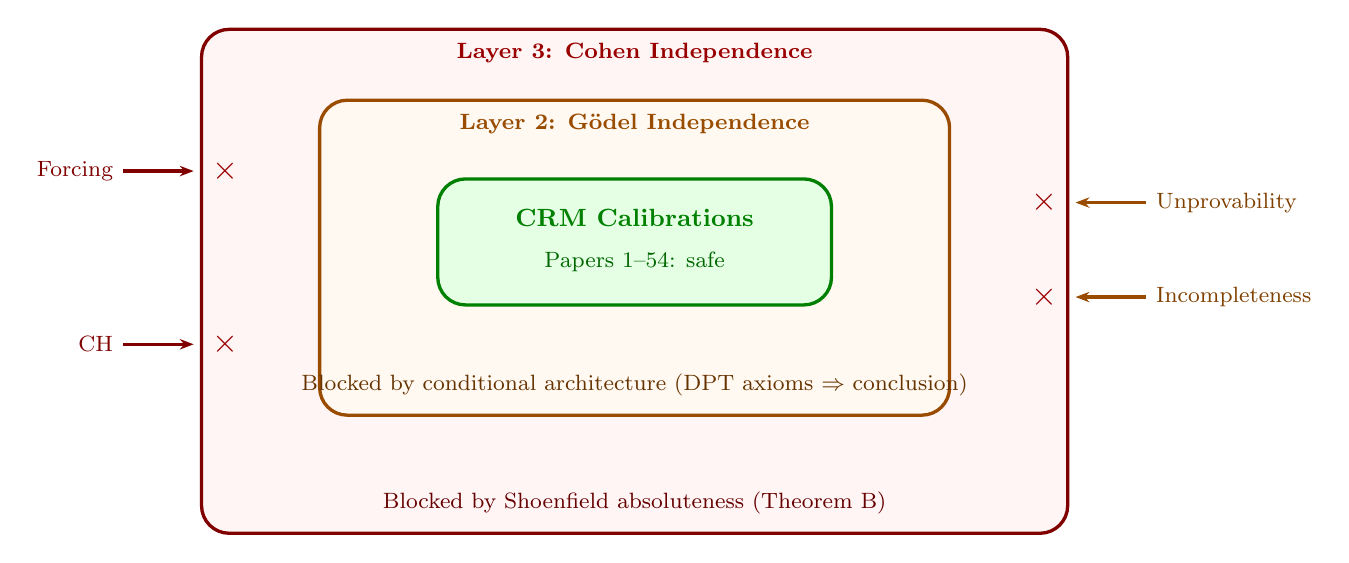
\begin{tikzpicture}[
  layer/.style={draw, very thick, rounded corners=10pt, align=center},
  blocked/.style={font=\footnotesize\bfseries, text=red!60!black},
  threat/.style={-{Stealth[length=5pt]}, very thick},
  cross/.style={font=\large\bfseries, text=red!60!black}
]
  % Layer 3 (outermost): Cohen independence
  \node[layer, draw=red!50!black, fill=red!4,
        minimum width=11cm, minimum height=6.4cm] (L3) at (0,0) {};
  \node[blocked, anchor=north] at ([yshift=-2pt]L3.north) {Layer 3: Cohen Independence};
  \node[font=\footnotesize, text=red!40!black, anchor=south] at ([yshift=4pt]L3.south)
    {Blocked by Shoenfield absoluteness (Theorem~B)};

  % Layer 2 (middle): Gödel independence
  \node[layer, draw=orange!60!black, fill=orange!5,
        minimum width=8cm, minimum height=4.0cm] (L2) at (0,0.3) {};
  \node[font=\footnotesize\bfseries, text=orange!60!black, anchor=north] at ([yshift=-2pt]L2.north)
    {Layer 2: G\"odel Independence};
  \node[font=\footnotesize, text=orange!40!black, anchor=south] at ([yshift=4pt]L2.south)
    {Blocked by conditional architecture (DPT axioms $\Rightarrow$ conclusion)};

  % Layer 1 (innermost): CRM calibrations
  \node[layer, draw=green!50!black, fill=green!10,
        minimum width=5cm, minimum height=1.6cm] (L1) at (0,0.5) {};
  \node[font=\small\bfseries, text=green!50!black] at (0,0.8)
    {CRM Calibrations};
  \node[font=\footnotesize, text=green!40!black] at (0,0.25)
    {Papers 1--54: safe};

  % Threat arrows with X marks
  \draw[threat, red!50!black] (-6.5,1.4) -- (-5.6,1.4);
  \node[cross] at (-5.2,1.4) {$\times$};
  \node[font=\footnotesize, text=red!50!black, left] at (-6.5,1.4) {Forcing};

  \draw[threat, red!50!black] (-6.5,-0.8) -- (-5.6,-0.8);
  \node[cross] at (-5.2,-0.8) {$\times$};
  \node[font=\footnotesize, text=red!50!black, left] at (-6.5,-0.8) {$\CH$};

  \draw[threat, orange!60!black] (6.5,1.0) -- (5.6,1.0);
  \node[cross] at (5.2,1.0) {$\times$};
  \node[font=\footnotesize, text=orange!50!black, right] at (6.5,1.0)
    {Unprovability};

  \draw[threat, orange!60!black] (6.5,-0.2) -- (5.6,-0.2);
  \node[cross] at (5.2,-0.2) {$\times$};
  \node[font=\footnotesize, text=orange!50!black, right] at (6.5,-0.2)
    {Incompleteness};
\end{tikzpicture}
\caption{The three layers of CRM program insulation (Proposition~\ref{prop:audit}).
External threats---Cohen forcing and G\"odel incompleteness---are blocked
at successive barriers.  The conditional architecture ensures that
calibration results hold regardless of the provability status of
Conjecture~D.}
\label{fig:insulation}
\end{figure}


%% ===================================================================
\section{CRM Audit}
\label{sec:crm}
%% ===================================================================

\subsection{Constructive strength classification}

\begin{center}
\renewcommand{\arraystretch}{1.3}
\begin{tabular}{llll}
\toprule
\textbf{Result} & \textbf{Strength} & \textbf{Status} & \textbf{Axioms} \\
\midrule
Theorem A (arithmetical classification) & $\BISH$ (encoding) & Structural & None (definition) \\
Theorem B (Cohen immunity) & $\BISH$ (implication) & Proved & Shoenfield (axiomatized) \\
Theorem C (G\"odel gap) & $\BISH$ (implication) & Proved & G\"odel (axiomatized) \\
CRM insulation & $\BISH$ (implication) & Proved & None \\
\bottomrule
\end{tabular}
\end{center}

\smallskip\noindent
Every result in this paper operates at the level of pure logic ($\BISH$): no omniscience principle is needed, no excluded middle is invoked.  The theorems are \emph{about} the logical status of Conjecture~D, not proofs \emph{of} Conjecture~D.  The deep external theorems (Shoenfield absoluteness, G\"odel's second incompleteness) are axiomatized as hypotheses; the logical implications are fully proved.

\subsection{The descent pattern and Paper 55's place}

The CRM program exhibits a consistent \emph{de-omniscientizing descent} pattern across the series:
\begin{center}
\renewcommand{\arraystretch}{1.3}
\begin{tabular}{lll}
\toprule
\textbf{Paper} & \textbf{Domain} & \textbf{Descent} \\
\midrule
Paper~2 & Banach spaces & $\WLPO \to \BISH$ (reflexive bypass) \\
Paper~8 & Ising model & $\LPO \to \BISH$ (transfer matrix) \\
Paper~26 & Bidual gap & $\WLPO$-complete (G\"odel sequences) \\
Paper~40 & Spectral gap & $\LPO$-complete (Wang tiling) \\
Paper~45 & WMC & $\LPO \to \BISH$ (geometric descent) \\
Paper~55 & Conjecture~D meta-level & Cohen ruled out; G\"odel confined \\
\bottomrule
\end{tabular}
\end{center}

\smallskip\noindent
Paper~55 extends the audit to the \emph{meta-mathematical} level: rather than calibrating a mathematical theorem against omniscience principles, it calibrates the \emph{provability} of a theorem against modes of independence.  The result---Cohen independence is impossible, G\"odel independence is confined but open---mirrors the descent pattern: set-theoretic independence (the ``strongest'' mode) is eliminated, leaving only the arithmetical residue.


%% ===================================================================
\section{Formal Verification}
\label{sec:formal}
%% ===================================================================

\subsection{File structure and build status}

The Lean~4 bundle resides at \texttt{paper~55/P55\_GoedelConjD/} with the following structure:

\begin{center}
\begin{tabular}{lll}
\toprule
\textbf{File} & \textbf{Lines} & \textbf{Content} \\
\midrule
\texttt{Defs.lean} & 191 & Arithmetical hierarchy, formal systems, models, two \\
& & modes of independence, ConjDData, DPT axioms \\
\texttt{Absoluteness.lean} & 117 & Shoenfield absoluteness, Cohen immunity, \\
& & G\"odel gap (absoluteness $\neq$ provability) \\
\texttt{CohenImmunity.lean} & 146 & CRM insulation, classification, mutual \\
& & exclusivity of Cohen vs G\"odel independence \\
\texttt{Main.lean} & 104 & Root module + \texttt{\#print axioms} audit \\
\bottomrule
\end{tabular}
\end{center}

\medskip\noindent
\textbf{Build status:} \texttt{lake build} $\to$ \textbf{0 errors, 0 warnings, 0 \texttt{sorry}s}.  Lean~4 version: \texttt{v4.29.0-rc1}.  Mathlib4 dependency via \texttt{lakefile.lean}.  Reproducible from Zenodo.

\subsection{Axiom inventory}

The formalization uses \textbf{zero custom axioms}.  All mathematical content (Shoenfield absoluteness, G\"odel's incompleteness, the~$\Pi^0_2$ form of Conjecture~D) is modeled via Lean structures that are passed as \emph{hypotheses} to theorems, not as global axioms.

\textbf{Scope and limitations.}  The Lean bundle verifies the \emph{logical plumbing}: the chain of implications from arithmetical classification through Shoenfield absoluteness to Cohen immunity, the gap between absoluteness and provability, and the mutual exclusivity of the two modes of independence.  It does \emph{not} verify the mathematical content that feeds into the architecture---the computability of cycle classes, the spreading-out reduction, or Shoenfield's theorem itself.  These are axiomatized as hypotheses.  The formalization uses a single \texttt{Pi02Sentence} type and does not distinguish the~$\Pi^0_3$ degradation in positive characteristic; both~$\Pi^0_2$ and~$\Pi^0_3$ are arithmetical and hence $\Sigma^1_2$, so the logical chain (arithmetical $\Rightarrow$ $\Sigma^1_2$ $\Rightarrow$ Shoenfield-absolute) is verified uniformly.  The formalization certifies that \emph{if} the mathematical inputs are correct, the logical conclusions follow.  That eight of ten theorems use no Lean axioms reflects the propositional character of the implications, not the depth of the verification.  The reader should view the Lean bundle as a consistency check on the paper's logical structure, not as an independent contribution.

\begin{center}
\small
\begin{tabular}{lll}
\toprule
\textbf{Structure} & \textbf{Role} & \textbf{Models} \\
\midrule
\texttt{Pi02Sentence} & $\Pi^0_2$ sentence with decidable $R$ & Conjecture~D \\
\texttt{Pi01Sentence} & $\Pi^0_1$ sentence & $\Con(\ZFC)$ \\
\texttt{FormalSystem} & Formal system with soundness & $\ZFC$, $\PA$ \\
\texttt{TransitiveModel} & Transitive model of $\ZFC$ & $V$, $V[G]$ \\
\texttt{ShoenfieldAbsoluteness} & Absoluteness hypothesis & Shoenfield's theorem \\
\texttt{GoedelSecondIncompleteness} & Incompleteness hypothesis & G\"odel's theorem \\
\texttt{ConjDData} & Conj.~D as $\Pi^0_2$ sentence & Geometric encoding \\
\texttt{DPTAxioms} & CRM conditional hypotheses & Papers~51--53 \\
\texttt{CRMConditional} & Motive kills LPO & CRM main result \\
\bottomrule
\end{tabular}
\end{center}

\subsection{Key code snippets}

\textbf{Cohen immunity} (full proof, Absoluteness.lean):

\begin{lstlisting}
theorem conjD_cohen_immune
    (data : ConjDData)
    (SA : ShoenfieldAbsoluteness) :
    ¬ cohen_independent data.conjD SA.zfc_models := by
  have h_abs : absolute data.pi02_form.statement
      SA.zfc_models :=
    SA.pi02_absolute data.pi02_form
  have h_eq : data.pi02_form.statement = data.conjD :=
    data.captures
  rw [← h_eq]
  exact absolute_not_cohen_independent _ _ h_abs
\end{lstlisting}

\textbf{The G\"odel gap} (full proof, Absoluteness.lean):

\begin{lstlisting}
theorem absoluteness_not_implies_provability
    (G : GoedelSecondIncompleteness)
    (SA : ShoenfieldAbsoluteness) :
    ∃ φ : Pi02Sentence,
      absolute φ.statement SA.zfc_models ∧
      independent G.T φ.statement := by
  exact ⟨G.conT.toPi02,
    SA.pi02_absolute G.conT.toPi02,
    ⟨G.unprovable, G.unrefutable⟩⟩
\end{lstlisting}

\textbf{CRM insulation} (full proof, CohenImmunity.lean):

\begin{lstlisting}
theorem crm_conditional_independent_of_provability
    (cond : CRMConditional)
    (_T : FormalSystem) :
    (cond.dpt.decidable_equality →
     cond.dpt.algebraic_spectrum →
     cond.dpt.archimedean_polarization →
     (cond.lpo → cond.mp)) := by
  exact cond.motive_kills_lpo
\end{lstlisting}

\textbf{Mutual exclusivity} (full proof, CohenImmunity.lean):

\begin{lstlisting}
theorem modes_mutually_exclusive (T : FormalSystem)
    (φ : Prop)
    (models : TransitiveModel → Prop) :
    goedel_independent T φ models →
    ¬ cohen_independent φ models := by
  intro h_goedel h_cohen
  exact absolute_not_cohen_independent
    φ models h_goedel.1 h_cohen
\end{lstlisting}

\subsection{\texttt{\#print axioms} output}

\begin{center}
\small
\begin{tabular}{ll}
\toprule
\textbf{Theorem} & \textbf{Axioms} \\
\midrule
\texttt{absolute\_not\_cohen\_independent} & (no axioms) \\
\texttt{conjD\_cohen\_immune} & (no axioms) \\
\texttt{goedel\_independent\_witness} & \texttt{[propext]} \\
\texttt{absoluteness\_not\_implies\_provability} & \texttt{[propext]} \\
\texttt{crm\_conditional\_independent\_of\_provability} & (no axioms) \\
\texttt{modes\_mutually\_exclusive} & (no axioms) \\
\texttt{cohen\_independent\_not\_absolute} & (no axioms) \\
\texttt{goedel\_independent\_is\_absolute} & (no axioms) \\
\texttt{mkInsulation} & (no axioms) \\
\texttt{mkClassification} & (no axioms) \\
\bottomrule
\end{tabular}
\end{center}

\medskip\noindent
\textbf{Classical.choice audit.}  No theorem in this bundle uses \texttt{Classical.choice}.  Eight of ten theorems use \emph{no axioms at all}---they are pure logical implications.  The remaining two (\texttt{goedel\_independent\_witness} and \texttt{absoluteness\_not\_implies\_provability}) use only \texttt{propext} (propositional extensionality), which appears when rewriting along propositional equalities in the G\"odel incompleteness argument.

The minimal axiom profile is a natural consequence of the paper's subject matter, not an achievement of the formalization: since the theorems are logical implications with axiomatized hypotheses, Lean has very little to do.  Unlike Papers~2--45, which operate over~$\R$ or~$\C$ (where Mathlib's Cauchy completion infrastructure forces \texttt{Classical.choice} into every theorem), Paper~55 works entirely at the level of propositional logic and natural number arithmetic, where no classical infrastructure is needed.

\subsection{Reproducibility}

The Lean bundle will be archived at Zenodo with a permanent DOI.  To reproduce:
\begin{enumerate}[nosep]
\item Install Lean~4 (\texttt{v4.29.0-rc1}) and \texttt{lake}.
\item Clone the bundle from Zenodo.
\item Run \texttt{lake build} in the \texttt{P55\_GoedelConjD/} directory.
\item Verify: 0 errors, 0 warnings, 0 \texttt{sorry}s.
\end{enumerate}


%% ===================================================================
\section{Discussion}
\label{sec:discuss}
%% ===================================================================

\subsection{The arithmetical hierarchy and the CRM hierarchy}

The analysis reveals a structural parallel between two hierarchies:

\begin{center}
\renewcommand{\arraystretch}{1.3}
\begin{tabular}{lll}
\toprule
\textbf{Arithmetical hierarchy} & \textbf{CRM hierarchy} & \textbf{Character} \\
\midrule
$\Delta^0_0$ (decidable)        & $\BISH$ (finite computation)  & Algorithmic \\
$\Pi^0_1$ ($\forall n\, R(n)$)  & $\WLPO$ (detect zero sequence)& Oracle: detect \\
$\Sigma^0_1$ ($\exists n\, R(n)$) & $\LPO$ (decide $\exists n\, R(n)$) & Oracle: search \\
--- & $\MP$ ($\lnot\lnot\exists \to \exists$) & Witness: actualize \\
$\Sigma^1_2$ (Shoenfield limit) & $\CLASS$ (full excluded middle) & Unrestricted \\
\bottomrule
\end{tabular}
\end{center}

\emph{Reading the table.}  $\LPO$ decides $\forall\alpha \,[\alpha = 0 \lor \exists n\, (\alpha(n) = 1)]$, which is a~$\Sigma^0_1$ oracle (halting oracle).  $\WLPO$ decides $\forall\alpha \,[\alpha = 0 \lor \alpha \ne 0]$ without locating a witness, a~$\Pi^0_1$ oracle.  $\MP$ extracts an existential witness from a double negation ($\lnot\lnot\exists n \to \exists n$) and does not correspond cleanly to a single level of the arithmetical hierarchy---it sits ``between'' $\WLPO$ and $\LPO$ in oracle strength but on an independent axis.

This parallel is heuristic and should not be over-interpreted: the arithmetical hierarchy classifies \emph{sentences} by quantifier complexity, while the CRM hierarchy classifies \emph{principles} by the oracle strength they assert.  The two hierarchies live in different categories and there is no known theorem relating $\Pi^0_n$ complexity to a specific CRM level in general.  Nevertheless, the alignment is suggestive: $\LPO$ is the~$\Sigma^0_1$ decision oracle, and the spectral gap undecidability (Paper~40) was shown to be $\Sigma^0_1$-complete, consistent with its $\LPO$-equivalence in the CRM hierarchy.  Conjecture~D sits at~$\Pi^0_2$ (characteristic~$0$), and the motive's role is to \emph{descend} from the~$\LPO$ level to~$\MP$ (or~$\BISH$) by providing algebraic structure that bounds the existential witness search.

\subsection{Connection to Paper~40: undecidability genealogy and the two ceilings}

Paper~40~\cite{Paper40} advanced the thesis that all physical undecidability (among the results calibrated in the series) traces to a single source---Wang tiling---and saturates at exactly $\BISH + \LPO$.  (This is a thesis about the currently calibrated physics, not a proved metatheorem; see Paper~54~\cite{Paper54}, \S3.)  The Cubitt--Perez-Garcia--Wolf spectral gap undecidability~\cite{CubittPW2015} was classified as $\Sigma^0_1$-complete (computational complexity); Paper~36 gave the CRM calibration as $\LPO$-equivalent (constructive logical strength).  The bridge between the two frameworks is the identification of~$\LPO$ as the~$\Sigma^0_1$ decision oracle---an informal but structurally grounded correspondence, not a formal theorem.

Paper~40 identified two ceilings:
\begin{enumerate}[nosep]
\item \textbf{Empirical ceiling} ($\Sigma^0_1 / \LPO$): the level at which physical undecidability saturates.
\item \textbf{Platonic ceiling} ($\Sigma^0_2$): the level of empirically inaccessible truths.
\end{enumerate}
Conjecture~D, as a~$\Pi^0_2$ sentence (in characteristic~$0$), sits at the \emph{Platonic} ceiling---its $\forall\exists$ quantifier structure matches the complexity of idealized intensive observables---\emph{not} at the empirical ceiling ($\Sigma^0_1$).  The spectral gap problem ($\Sigma^0_1$-complete) sits at the empirical ceiling.  The G\"odel question---whether~$\ZFC$'s induction axioms suffice to bound the witness search in the~$\Pi^0_2$ formulation---resides at the boundary between the two ceilings (Figure~\ref{fig:ceilings}).  If Conjecture~D is provable in~$\ZFC$, the witness function is provably total and the sentence effectively collapses to the empirical level; if not, it remains at the Platonic level.

\begin{figure}[ht]
\centering
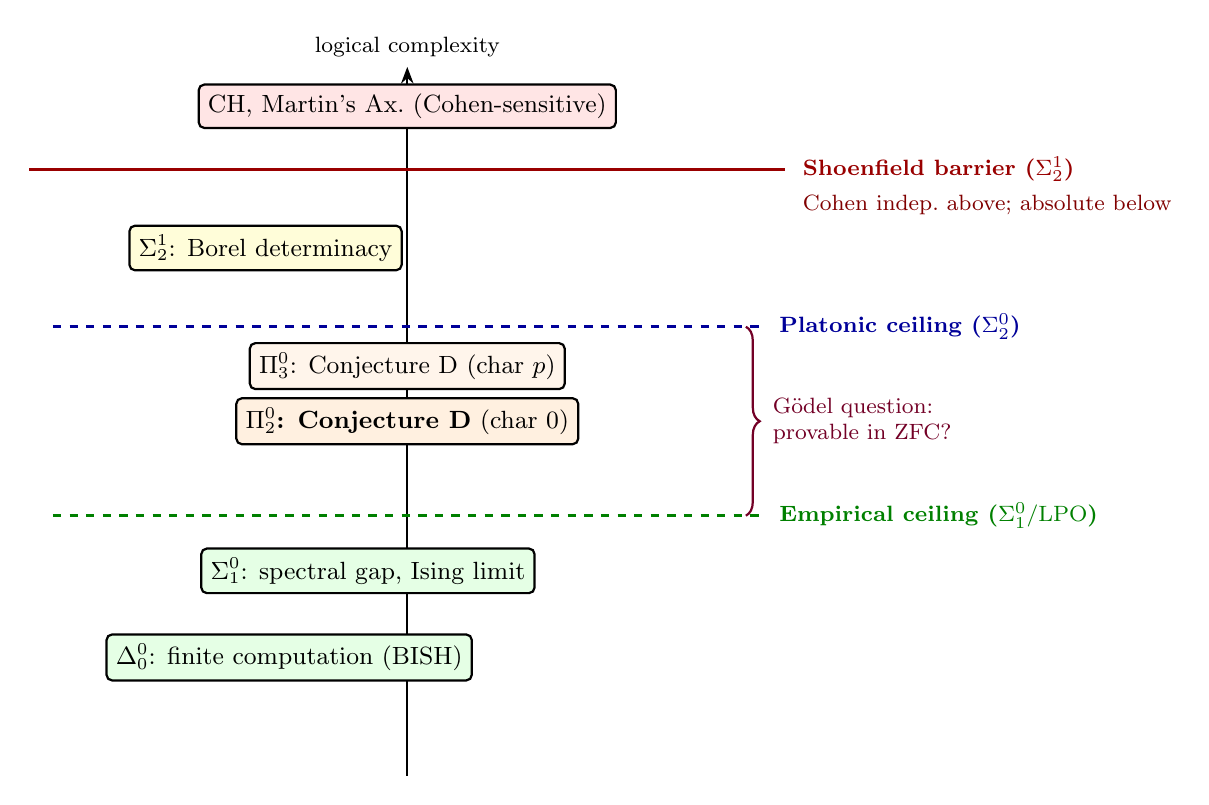
\begin{tikzpicture}[
  ceil/.style={very thick, dashed},
  item/.style={font=\small, align=left},
  barrier/.style={very thick, red!60!black}
]
  % Vertical axis
  \draw[-{Stealth[length=6pt]}, thick] (0,-0.5) -- (0,8.5)
    node[above, font=\footnotesize] {logical complexity};

  % Shoenfield barrier at top
  \draw[barrier] (-4.8,7.2) -- (4.8,7.2);
  \node[font=\footnotesize\bfseries, text=red!60!black, right] at (4.9,7.2)
    {Shoenfield barrier ($\Sigma^1_2$)};
  \node[font=\footnotesize, text=red!50!black, right] at (4.9,6.75)
    {Cohen indep.\ above; absolute below};

  % Platonic ceiling
  \draw[ceil, blue!60!black] (-4.5,5.2) -- (4.5,5.2);
  \node[font=\footnotesize\bfseries, text=blue!60!black, right] at (4.6,5.2)
    {Platonic ceiling ($\Sigma^0_2$)};

  % Empirical ceiling
  \draw[ceil, green!50!black] (-4.5,2.8) -- (4.5,2.8);
  \node[font=\footnotesize\bfseries, text=green!50!black, right] at (4.6,2.8)
    {Empirical ceiling ($\Sigma^0_1 / \LPO$)};

  % Items placed at levels
  \node[item, fill=green!10, draw, rounded corners=2pt, thick]
    at (-1.5,1.0) {$\Delta^0_0$: finite computation ($\BISH$)};

  \node[item, fill=green!10, draw, rounded corners=2pt, thick]
    at (-0.5,2.1) {$\Sigma^0_1$: spectral gap, Ising limit};

  \node[item, fill=orange!12, draw, rounded corners=2pt, thick]
    at (0,4.0) {\textbf{$\Pi^0_2$: Conjecture D} (char $0$)};

  \node[item, fill=orange!8, draw, rounded corners=2pt, thick]
    at (0,4.7) {$\Pi^0_3$: Conjecture D (char $p$)};

  \node[item, fill=yellow!15, draw, rounded corners=2pt, thick]
    at (-1.8,6.2) {$\Sigma^1_2$: Borel determinacy};

  \node[item, fill=red!10, draw, rounded corners=2pt, thick]
    at (0,8.0) {CH, Martin's Ax.\ (Cohen-sensitive)};

  % Brace for "G\"odel question" zone
  \draw[decorate, decoration={brace, amplitude=5pt, mirror}, thick, purple!60!black]
    (4.3,2.8) -- (4.3,5.2)
    node[midway, right=6pt, font=\footnotesize, text=purple!60!black, align=left]
    {G\"odel question:\\provable in $\ZFC$?};
\end{tikzpicture}
\caption{The two ceilings and the Shoenfield barrier.  Physical undecidability
saturates at the empirical ceiling ($\Sigma^0_1 / \LPO$).  Conjecture~D sits
at the Platonic ceiling ($\Pi^0_2$).  Everything below the Shoenfield barrier
($\Sigma^1_2$) is immune to Cohen independence.  The residual G\"odel question
occupies the zone between the two ceilings.}
\label{fig:ceilings}
\end{figure}

\subsection{Connection to Paper~26: G\"odel sequences and WLPO-completeness}

Paper~26~\cite{Paper26} embedded G\"odel's incompleteness into functional analysis.  The construction: for a $\Pi^0_1$ sentence~$\varphi$, define $v^\varphi(k) = 1$ if bounded proof search for~$\lnot\varphi$ fails by step~$k$, yielding a sequence in~$\ell^\infty$.  Whether $v^\varphi \in c_0$ (gap absent) or $v^\varphi \notin c_0$ (gap present) encodes the consistency of~$\varphi$, establishing the calibration chain:
\[
  \WLPO \;\;\leftrightarrow\;\; \Pi^0_1\text{-consistency decidable} \;\;\leftrightarrow\;\; \text{gap detection decidable}.
\]

Paper~55 addresses the next level up.  Where Paper~26 showed that $\Pi^0_1$ sentences (like $\Con(\ZFC)$) embed into the $\WLPO$ stratum, the present paper shows that Conjecture~D---a~$\Pi^0_2$ sentence in characteristic~$0$---sits above the empirical ceiling but still within the arithmetical world.  The relationship is:
\begin{center}
\renewcommand{\arraystretch}{1.3}
\begin{tabular}{llll}
\toprule
\textbf{Paper} & \textbf{Sentence type} & \textbf{CRM level} & \textbf{Example} \\
\midrule
Paper~26 & $\Pi^0_1$ & $\WLPO$ & $\Con(\ZFC)$ \\
Paper~40 & $\Sigma^0_1$ & $\LPO$ & Spectral gap \\
Paper~55 & $\Pi^0_2 / \Pi^0_3$ & Above $\LPO$, arithmetical & Conjecture~D \\
\bottomrule
\end{tabular}
\end{center}

\noindent Note that Conjecture~D's~$\Pi^0_2$ complexity does not correspond directly to the CRM level~$\LPO$; rather,~$\LPO$ is the~$\Sigma^0_1$ oracle, and~$\Pi^0_2$ sits one quantifier alternation higher.  The motive's role (Papers~45--53) is to reduce the CRM strength of Conjecture~D's \emph{consequences} from~$\LPO$ to~$\MP$, not to reduce the arithmetical complexity of the sentence itself.

The crucial difference: Paper~26's G\"odel sequences are \emph{known} to encode independent sentences ($\Con(\ZFC)$ is independent of~$\ZFC$), while Paper~55 shows that Conjecture~D \emph{could} be independent but is more likely provable.  The G\"odel phenomenon is a proven fact at~$\Pi^0_1$ (the $\WLPO$ level) but only a logical possibility at~$\Pi^0_2$.

\subsection{Convergence of the three prior programs}

The three research programs surveyed in \S\ref{sec:intro} converge on the provability question from complementary angles:

\begin{enumerate}[nosep]
\item \textbf{Friedman's Grand Conjecture}~\cite{Friedman1999}, if true, would settle the matter entirely: Conjecture~D would be provable in~$\EFA$, far below~$\ZFC$.

\item \textbf{McLarty's results}~\cite{McLarty2020} show that the \emph{machinery} of algebraic geometry lives in finite-order arithmetic---but the \emph{truth} of Conjecture~D requires that machinery to succeed for every variety, which is a separate question.

\item \textbf{Macintyre's first-order analysis}~\cite{Macintyre2003} of Weil cohomology opens the door to model-theoretic approaches: could one construct a non-standard model of~$\PA$ in which a ``variety'' violates~D?
\end{enumerate}

All three confirm that Conjecture~D inhabits the arithmetical world, but none closes the provability question.  The present paper adds the fourth angle: Shoenfield absoluteness eliminates the set-theoretic mode of independence, confining the question to the arithmetical mode (Figure~\ref{fig:convergence}).

\begin{figure}[ht]
\centering
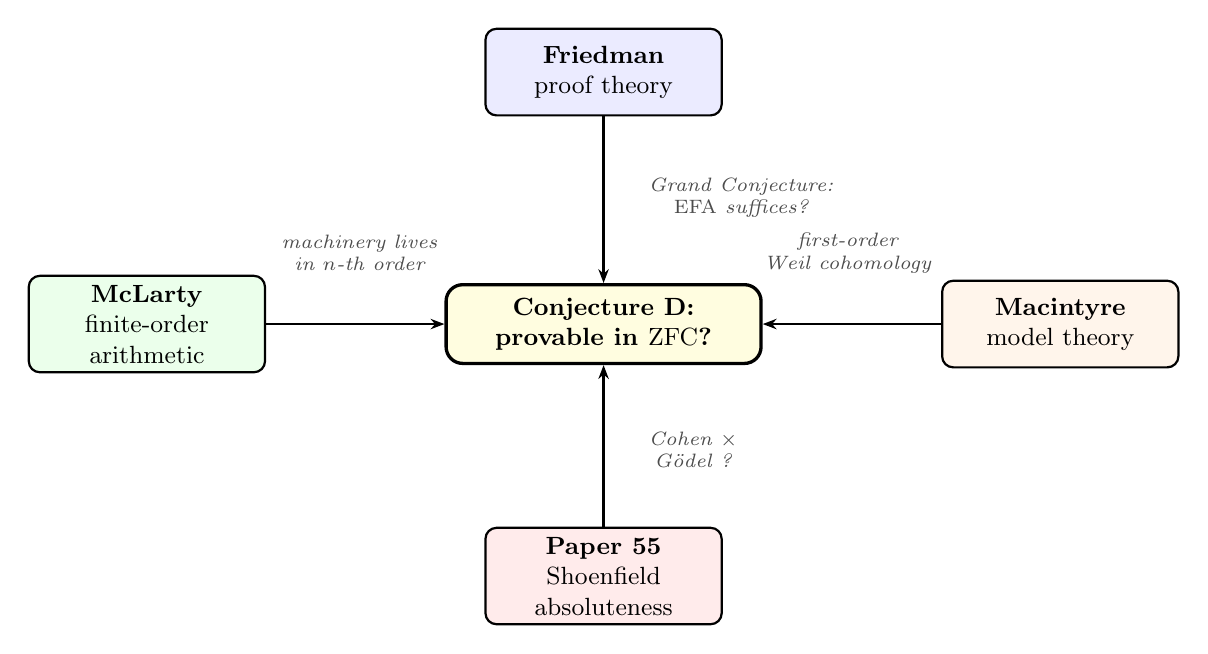
\begin{tikzpicture}[
  prog/.style={draw, rounded corners=4pt, thick, minimum width=3.0cm,
               minimum height=1.1cm, align=center, font=\small},
  center/.style={draw, very thick, rounded corners=6pt, minimum width=4.0cm,
                 minimum height=1.0cm, align=center, font=\small\bfseries,
                 fill=yellow!12},
  arr/.style={-{Stealth[length=5pt]}, thick},
  annot/.style={font=\scriptsize\itshape, text=gray!60!black, align=center}
]
  % Central question
  \node[center] (Q) at (0,0) {Conjecture D:\\provable in $\ZFC$?};

  % Friedman (top)
  \node[prog, fill=blue!8] (F) at (0,3.2)
    {\textbf{Friedman}\\proof theory};
  \draw[arr] (F) -- (Q);
  \node[annot, right=10pt] at (0.1,1.6) {Grand Conjecture:\\$\EFA$ suffices?};

  % McLarty (left)
  \node[prog, fill=green!8] (M) at (-5.8,0)
    {\textbf{McLarty}\\finite-order\\arithmetic};
  \draw[arr] (M) -- (Q);
  \node[annot] at (-3.1,0.9) {machinery lives\\in $n$-th order};

  % Macintyre (right)
  \node[prog, fill=orange!8] (Mac) at (5.8,0)
    {\textbf{Macintyre}\\model theory};
  \draw[arr] (Mac) -- (Q);
  \node[annot] at (3.1,0.9) {first-order\\Weil cohomology};

  % Paper 55 (bottom)
  \node[prog, fill=red!8] (P55) at (0,-3.2)
    {\textbf{Paper 55}\\Shoenfield\\absoluteness};
  \draw[arr] (P55) -- (Q);
  \node[annot, right=10pt] at (0.1,-1.6) {Cohen $\times$\\G\"odel~?};
\end{tikzpicture}
\caption{Four complementary approaches to the provability question
for Standard Conjecture~D.  Each program confirms that~D inhabits the
arithmetical world; none closes the provability gap.}
\label{fig:convergence}
\end{figure}

\subsection{Why G\"odel almost never touches real mathematics or physics}

The analysis of Conjecture~D illustrates a broader phenomenon: G\"odel incompleteness, despite its foundational fame, has almost no impact on the practice of mathematics or physics.  This observation is not new---Feferman~\cite{Feferman2006} and Simpson~\cite{Simpson2009} have made the case from the proof-theoretic side---but the Shoenfield-based explanation may clarify the mechanism.  The explanation has three layers, which we now develop.

\medskip\noindent
\textbf{Layer 1: The Shoenfield barrier.}  Shoenfield's absoluteness theorem (Theorem~\ref{thm:shoenfield}) draws a sharp line through the logical universe.  Every sentence below~$\Sigma^1_2$---which includes \emph{every arithmetical sentence} ($\Pi^0_n$, $\Sigma^0_n$ for all~$n$) and even some analytic sentences (those with a single existential set quantifier followed by a universal set quantifier)---has its truth value determined by the natural numbers alone.  Set-theoretic independence (Cohen forcing, large cardinals, the Continuum Hypothesis) cannot touch any of these sentences.

The overwhelming majority of theorems in number theory, algebra, combinatorics, analysis, and physics are arithmetical or $\Sigma^1_2$ at most.  Fermat's Last Theorem is~$\Pi^0_1$.  The Riemann Hypothesis is~$\Pi^0_1$.  The Goldbach Conjecture is~$\Pi^0_1$.  The Birch and Swinnerton-Dyer Conjecture (for a fixed curve) is arithmetical.  The Navier--Stokes regularity problem, once formalized, sits in the analytic hierarchy but well within~$\Sigma^1_2$.  Conjecture~D is~$\Pi^0_2$ in characteristic~$0$ ($\Pi^0_3$ in positive characteristic).  \emph{All of these are immune to Cohen independence.}  The Continuum Hypothesis, Martin's Axiom, the existence or non-existence of large cardinals---none of these set-theoretic principles can affect the truth of any of these statements.

This is why set-theoretic independence results (Cohen 1963, Solovay, Easton, etc.) never intrude on number theory, algebraic geometry, or mathematical physics: the theorems of these fields live below the Shoenfield barrier.

\emph{Physics is even more protected than pure mathematics.}  Paper~40~\cite{Paper40} proved that all physical undecidability saturates at exactly~$\BISH + \LPO$, with every instance tracing to Wang tiling ($\Sigma^0_1$-complete).  The equations of physics---Maxwell, Schr\"odinger, Einstein, Yang--Mills---are differential equations whose well-posedness and regularity properties are at most~$\Sigma^1_2$.  The Cubitt--Perez-Garcia--Wolf spectral gap undecidability~\cite{CubittPW2015}, the strongest known undecidability result in physics, is~$\Sigma^0_1$: it asks whether a Turing machine (encoding the Hamiltonian's ground state gap) halts.  No physical theory has ever produced a statement above the Shoenfield barrier, nor is there a mechanism by which one could---physical observables are real-valued functions of finitely many parameters, not arbitrary subsets of uncountable sets.  G\"odel's theorems are not merely irrelevant to physics in practice; they are \emph{structurally excluded} by the arithmetical character of physical law.

\medskip\noindent
\textbf{Layer 2: The arithmetical barrier.}  Shoenfield eliminates Cohen independence but leaves G\"odel independence open.  Yet G\"odel independence is also extremely rare in practice.  Why?

The canonical example of G\"odel independence---$\Con(\ZFC)$---is a sentence \emph{about formal systems}, not about mathematical objects.  It asks whether a particular Turing machine (the proof-checker for~$\ZFC$) halts on a particular input (a proof of~$0 = 1$).  This is a metamathematical statement: a statement about the syntax of mathematics, not about its objects.

Theorems of ``real mathematics''---the Fundamental Theorem of Calculus, the Prime Number Theorem, the classification of finite simple groups, the Atiyah--Singer index theorem---are \emph{about mathematical objects}: functions, primes, groups, operators.  These objects have concrete structure (finite generation, geometric meaning, physical interpretation) that provides \emph{witnesses} for the existential quantifiers in their~$\Pi^0_2$ or~$\Sigma^0_1$ formulations.  The witnesses are constructible from the objects themselves, not from abstract proof search through formal systems.

G\"odel independence requires the witness search to outrun~$\ZFC$'s provable total functions---a growth rate faster than any function definable in~$\ZFC$.  This is characteristic of metamathematical and combinatorial pathologies (Friedman's Boolean relation theory~\cite{Friedman2001}, Paris--Harrington, Kanamori--McAloon) but not of theorems arising from geometry, analysis, or physics.  The structural richness of mathematical objects (algebraic cycles, smooth manifolds, self-adjoint operators) provides enough scaffolding to keep the witness search within~$\ZFC$'s reach.

\medskip\noindent
\textbf{Layer 3: What Hilbert's program got wrong.}  Hilbert's program (1920s) sought a \emph{finitary consistency proof} for all of mathematics.  G\"odel's theorems (1931) refuted this specific goal: no formal system can prove its own consistency, so there is no ``final foundation'' that validates itself.  This was a devastating blow to the \emph{foundational program}---the attempt to secure mathematics on a single, self-certifying formal system.

But Hilbert's program conflated two distinct questions (cf.~Detlefsen~\cite{Detlefsen1986}):
\begin{enumerate}[nosep]
\item \emph{Can mathematics validate its own consistency?}  (No---G\"odel.)
\item \emph{Can mathematics prove its own theorems?}  (Almost always yes---Shoenfield + practice.)
\end{enumerate}
The first question is about \emph{self-reference}: a formal system reasoning about itself, which triggers the diagonal argument.  The second question is about \emph{content}: a formal system reasoning about mathematical objects, which does not trigger self-reference because the objects (varieties, functions, operators) are not encodings of the system's own proof predicates.

G\"odel's theorems invalidate Hilbert's foundational aspiration but leave the \emph{working mathematician's} implicit program untouched.  The working mathematician does not need~$\ZFC$ to prove its own consistency; she needs~$\ZFC$ to prove theorems about algebraic curves, Banach spaces, and differential equations.  For this purpose, $\ZFC$ is (empirically and in every known case) sufficient.

\medskip\noindent
\textbf{Prior observations.}  The general principle that G\"odel's theorems are irrelevant to ordinary mathematics is not new.  Feferman~\cite{Feferman2006} argued that ``virtually all of scientifically applicable mathematics can be carried out'' in systems conservative over~$\PA$, and therefore that incompleteness phenomena have no bearing on mathematical practice.  Simpson's reverse mathematics program has long observed that most theorems of ``core mathematics'' are provable in subsystems of second-order arithmetic far weaker than~$\ZFC$.  What appears to be new is the specific three-layer explanation: (i)~the identification of Shoenfield absoluteness as the mechanism protecting all arithmetical sentences (not just an empirical observation that~$\ZFC$ suffices), (ii)~the explicit classification of major open conjectures by arithmetical complexity (placing FLT, RH, Goldbach, BSD, and Conjecture~D below the $\Sigma^1_2$ barrier), and (iii)~the framing of Hilbert's failure as a conflation of two questions rather than a refutation of one program.  Feferman's argument was proof-theoretic (what can~$\PA$ prove?); ours is model-theoretic (what does Shoenfield protect?) and adds the CRM hierarchy as a parallel stratification.

\medskip\noindent
\textbf{The CRM perspective.}  The CRM program provides a parallel framework.  The partial order $\BISH \subset \BISH + \LPO \subset \CLASS$ (with $\WLPO$ and $\MP$ as incomparable intermediate principles whose join is~$\LPO$) measures the ``oracle strength'' needed for a theorem.  G\"odel incompleteness enters at the $\WLPO$ level (Paper~26~\cite{Paper26}: $\Con(\ZFC)$ is~$\Pi^0_1$, which is the level of $\WLPO$), but its concrete instantiations are metamathematical (consistency statements).  Physical theorems saturate at~$\LPO$ (Paper~40~\cite{Paper40}), and algebraic geometry descends from~$\LPO$ to~$\MP$ via the motive (Papers~45--53).  The CRM program calibrates theorems against omniscience principles, not against provability in~$\ZFC$, so it does not directly test for G\"odel independence.  But the pattern is consistent: every theorem calibrated in the series has concrete geometric or analytic witnesses that keep it well within~$\ZFC$'s reach.

The present paper addresses the one place where the question becomes unavoidable: the meta-level provability of Conjecture~D itself.  The answer---Cohen-immune, and likely G\"odel-immune given the precedent from algebraic geometry---is consistent with the broader pattern.


\subsection{Comparison with Feferman's proof-theoretic approach}

Feferman's program~\cite{Feferman2006} is the most developed prior argument for the irrelevance of G\"odel's theorems to working mathematics.  It proceeds by \emph{proof-theoretic reduction}: Feferman and J\"ager (1993, 1996) proved that System~W (a predicative type theory for analysis) is conservative over~$\PA$ for arithmetic sentences, and Feferman demonstrated that separable analysis---Banach spaces, Hilbert spaces, measure theory---can be developed within~W.  The conclusion: since~$\PA$ suffices for the arithmetic content of scientifically applicable mathematics, G\"odel's incompleteness of~$\PA$ affects only metamathematical statements.

Our argument differs in tool, scope, and conclusion:

\begin{center}
\renewcommand{\arraystretch}{1.3}
\small
\begin{tabular}{lll}
\toprule
 & \textbf{Feferman} & \textbf{Paper~55} \\
\midrule
\textbf{Tool} & Proof theory (ordinal analysis) & Model theory (Shoenfield absoluteness) \\
\textbf{Central claim} & $\PA$ suffices for real math (thesis) & Arithmetical sentences are absolute (theorem) \\
\textbf{Cohen independence} & Not explicitly addressed & Formally ruled out (Theorem~B) \\
\textbf{G\"odel independence} & Implicitly irrelevant if $\PA$ suffices & Explicitly: possible but structurally distinct \\
\textbf{Status} & Core thesis is a \emph{conjecture} & Core results are \emph{theorems} \\
\textbf{Vulnerability} & Counterexamples exist (Borel det.) & None (Shoenfield is unconditional) \\
\bottomrule
\end{tabular}
\end{center}

\smallskip\noindent
The critical difference is that Feferman's central thesis---``all scientifically applicable mathematics can be carried out in~W''---is \emph{unproved and has known exceptions}.  Martin's Borel determinacy theorem (1975) requires uncountably many iterations of the powerset axiom, far exceeding~$\PA$.  The Cantor--Bendixson theorem is equivalent to~$\Pi^1_1$-$\mathrm{CA}_0$, whose proof-theoretic ordinal vastly exceeds~$\Gamma_0$.  Friedman's Boolean relation theory~\cite{Friedman2001} produces arithmetic statements independent of~$\ZFC$ itself.  These show genuine limits to the proof-theoretic approach.

Shoenfield absoluteness has no such vulnerability.  It is a \emph{theorem}, not a thesis, and it protects \emph{every} $\Sigma^1_2$ sentence unconditionally---regardless of whether~$\PA$, $\ZFC$, or $\ZFC$ plus large cardinals is needed to prove it.  Even if Conjecture~D requires large cardinal axioms to prove (an extreme scenario), its truth value is still the same in every transitive model.  Feferman's framework cannot express this: his tool measures what a system \emph{can prove}, not what is \emph{invariant across models}.

The two approaches are complementary, and each has an advantage the other lacks.  Feferman explains \emph{reduction} (how little formal strength is needed): when his thesis applies, it delivers a \emph{stronger} conclusion than ours---not merely that a sentence is absolute, but that it is provable in~$\PA$.  Absoluteness alone does not imply provability (the G\"odel gap), so Feferman's conclusion, where available, subsumes ours.  However, his thesis is a conjecture with known exceptions, while Shoenfield absoluteness is unconditional.  We explain \emph{protection} (what cannot be broken by set-theoretic methods): every $\Sigma^1_2$ sentence is protected, regardless of whether it is provable in~$\PA$, $\ZFC$, or only in $\ZFC$ plus large cardinals.  Both arrive at the same practical conclusion---G\"odel is irrelevant to working mathematics---but through different mechanisms.


\subsection{Why G\"odel independence is unlikely for Conjecture~D}

No major conjecture in algebraic geometry has been shown G\"odel-independent of~$\ZFC$.  The precedent strongly favors either proof (Fermat, Poincar\'e) or continued openness (Hodge, Riemann).  Several considerations suggest Conjecture~D is more likely provable:

\begin{enumerate}[nosep]
\item \textbf{Geometrically bounded witnesses.}  The witness cycle class~$[W]$ is evaluated against the numerical Chow group $\mathrm{CH}^{d-r}(X)_{\mathrm{num}} \otimes \Q$, which is a finite-dimensional $\Q$-vector space.  Unconditionally (not assuming~D), the rank of $\mathrm{CH}^r_{\mathrm{num}} \otimes \Q$ is bounded by the Betti number $\dim_\Q H^{2r}(X)$, since the non-degenerate intersection pairing on $\mathrm{CH}^r_{\mathrm{num}}$ and the comparison theorem give the bound.  The search for a witness~$W$ is bounded by this finite-rank lattice rather than over~$\N$ in the raw Peano sense, and the full Chow group $\mathrm{CH}^*(X)$---which is typically infinitely generated (cf.~Mumford's theorem for zero-cycles on surfaces)---need not be searched.

\item \textbf{Proven cases.}  Conjecture~D is known for abelian varieties~\cite{Lieberman1968}, surfaces (classical), and varieties with motivated cycles~\cite{Andre1996}.  Each proof uses concrete algebraic constructions, not strong set-theoretic axioms.

\item \textbf{Connection to other conjectures.}  The Hodge Conjecture implies Conjecture~D (in characteristic~$0$).  If the Hodge Conjecture is provable in~$\ZFC$, then so is Conjecture~D.
\end{enumerate}

However, ``unlikely'' is not ``impossible.''  The Friedman program has produced natural-looking combinatorial statements (e.g., Boolean relation theory~\cite{Friedman2001}) that are independent of~$\ZFC$.  A priori, we cannot rule out a similar phenomenon for Conjecture~D.

\subsection{Open questions}

\begin{enumerate}
\item Can the arithmetical classification be sharpened?  In characteristic~$0$, is Conjecture~D equivalent to a~$\Pi^0_1$ sentence (which would place it at the same level as $\Con(\ZFC)$ and in the Paper~26 stratum)?  In positive characteristic, can the~$\Pi^0_3$ classification be reduced to~$\Pi^0_2$ via an effective algorithm for $\ell$-adic cycle class computation?

\item Does a model-theoretic construction (in the spirit of Macintyre) yield a non-standard model of~$\PA$ where Conjecture~D fails?  This would establish G\"odel independence.

\item Does the CRM program's conditional architecture (DPT axioms) provide evidence for or against provability of Conjecture~D?  Specifically, are the DPT axioms themselves provable in~$\ZFC$?

\item Can the connection between the arithmetical hierarchy and the CRM hierarchy be made precise?  Is there a general theorem relating $\Pi^0_n$ complexity to the omniscience principle at the corresponding CRM level?
\end{enumerate}


%% ===================================================================
\section{Conclusion}
\label{sec:conclusion}
%% ===================================================================

We have organized known results from mathematical logic into a meta-mathematical audit of Standard Conjecture~D:

\begin{enumerate}
\item \textbf{Conjecture~D is arithmetical} (Theorem~A): $\Pi^0_2$ in characteristic~$0$, $\Pi^0_3$ in positive characteristic.  The proper class of all varieties collapses to a countable domain by spreading out and the Lefschetz principle.

\item \textbf{Set-theoretic independence is impossible} (Theorem~B).  By Shoenfield absoluteness, Conjecture~D has the same truth value in all transitive models of~$\ZFC$.  Forcing, $\CH$, and large cardinals are irrelevant.

\item \textbf{Arithmetical independence is not ruled out} (Theorem~C).  Conjecture~D could be true but unprovable in~$\ZFC$, in the same sense that $\Con(\ZFC)$ is true but unprovable.  This remains an open meta-mathematical question.
\end{enumerate}

The picture that emerges is reassuring for the CRM program: G\"odel is absent from the internal computations, absent from the set-theoretic meta-level, and confined---if present at all---to a purely arithmetical question about the inductive strength of~$\ZFC$.  The conditional architecture (DPT axioms) insulates all calibration results from both modes of independence.

None of the individual results are surprising to a logician familiar with Shoenfield absoluteness.  The value of this paper lies in the assembly: making the meta-mathematical status of the CRM program's foundations explicit, connecting the arithmetical classification of Conjecture~D to the prior programs of Macintyre, McLarty, and Friedman, and comparing the model-theoretic approach (Shoenfield) with the proof-theoretic approach (Feferman).  This completes the meta-mathematical audit initiated in Paper~54's \S7.2.


%% ===================================================================
\section*{Acknowledgments}
\addcontentsline{toc}{section}{Acknowledgments}
%% ===================================================================

The logical analysis in this paper was developed through dialogue with AI systems (Claude, Anthropic) that identified the key distinction between Cohen independence and G\"odel independence for arithmetical statements.  The geometric correction (direction of Conjecture~D) and the spreading-out reduction follow standard references.  All mathematical claims and errors remain the author's responsibility.

We thank the Mathlib contributors for the propositional logic and natural number arithmetic infrastructure.  The Lean~4 formalization was produced using AI code generation (Claude Code, Opus~4.6) under human direction.  The author is a practicing cardiologist rather than a professional logician or arithmetic geometer; all mathematical claims should be evaluated on their formal content.  We welcome constructive feedback from domain experts.


%% ===================================================================
% Bibliography
%% ===================================================================

\begin{thebibliography}{99}

\bibitem{Shoenfield1961}
J.~R.~Shoenfield.
\newblock The problem of predicativity.
\newblock In \emph{Essays on the Foundations of Mathematics}, pp.~132--139, 1961.

\bibitem{Kleiman1968}
S.~Kleiman.
\newblock Algebraic cycles and the Weil conjectures.
\newblock In \emph{Dix expos\'es sur la cohomologie des sch\'emas}, pp.~359--386, North-Holland, 1968.

\bibitem{Grothendieck1969}
A.~Grothendieck.
\newblock Standard conjectures on algebraic cycles.
\newblock In \emph{Algebraic Geometry, Bombay 1968}, pp.~193--199, Oxford University Press, 1969.

\bibitem{Lieberman1968}
D.~Lieberman.
\newblock Numerical and homological equivalence of algebraic cycles on Hodge manifolds.
\newblock \emph{Amer. J. Math.}, 90:366--374, 1968.

\bibitem{Andre1996}
Y.~Andr\'e.
\newblock Pour une th\'eorie inconditionnelle des motifs.
\newblock \emph{Publ. Math. IH\'ES}, 83:5--49, 1996.

\bibitem{OakuTakayama1999}
T.~Oaku and N.~Takayama.
\newblock An algorithm for de Rham cohomology groups of the complement of an affine variety via $D$-module computation.
\newblock \emph{J. Pure Appl. Algebra}, 139:201--233, 1999.

\bibitem{Goedel1931}
K.~G\"odel.
\newblock \"Uber formal unentscheidbare S\"atze der Principia Mathematica und verwandter Systeme~I.
\newblock \emph{Monatshefte f\"ur Mathematik und Physik}, 38:173--198, 1931.

\bibitem{Friedman2001}
H.~Friedman.
\newblock Long finite sequences.
\newblock \emph{J. Combin. Theory Ser. A}, 95(1):102--144, 2001.

\bibitem{Macintyre2003}
A.~Macintyre.
\newblock Model theory: Geometrical and set-theoretic aspects and prospects.
\newblock \emph{Bull. Symbolic Logic}, 9(2):197--212, 2003.

\bibitem{Zilber2010}
B.~Zilber.
\newblock \emph{Zariski Geometries: Geometry from the Logician's Point of View}.
\newblock LMS Lecture Note Series~360. Cambridge University Press, 2010.

\bibitem{Gavrilovich2018}
M.~Gavrilovich.
\newblock Standard conjectures in model theory, and categoricity of comparison isomorphisms.
\newblock \emph{arXiv:1808.09332}, 2018.

\bibitem{McLarty2010}
C.~McLarty.
\newblock What does it take to prove Fermat's Last Theorem? Grothendieck and the logic of number theory.
\newblock \emph{Bull. Symbolic Logic}, 16(3):359--377, 2010.

\bibitem{McLarty2020}
C.~McLarty.
\newblock The large structures of Grothendieck founded on finite-order arithmetic.
\newblock \emph{Rev. Symbolic Logic}, 13(2):296--325, 2020.

\bibitem{Friedman1999}
H.~Friedman.
\newblock Grand conjectures.
\newblock FOM mailing list, April 1999.
\newblock \url{https://cs.nyu.edu/pipermail/fom/1999-April/003014.html}

\bibitem{Avigad2003}
J.~Avigad.
\newblock Number theory and elementary arithmetic.
\newblock \emph{Philosophia Mathematica}, 11(3):257--284, 2003.

\bibitem{Detlefsen1986}
M.~Detlefsen.
\newblock \emph{Hilbert's Program: An Essay on Mathematical Instrumentalism}.
\newblock Synthese Library~182. Reidel, 1986.

\bibitem{Feferman2006}
S.~Feferman.
\newblock Are there absolutely unsolvable problems? G\"odel's dichotomy.
\newblock \emph{Philosophia Mathematica}, 14(2):134--152, 2006.

\bibitem{BridgesRichman1987}
D.~Bridges and F.~Richman.
\newblock \emph{Varieties of Constructive Mathematics}.
\newblock LMS Lecture Note Series~97. Cambridge University Press, 1987.

\bibitem{CubittPW2015}
T.~S.~Cubitt, D.~Perez-Garcia, and M.~M.~Wolf.
\newblock Undecidability of the spectral gap.
\newblock \emph{Nature}, 528:207--211, 2015.

\bibitem{Paper26}
P.~C.~K.~Lee.
\newblock Bidual gap detection is WLPO-complete: G\"odel sequences (Paper~26).
\newblock CRM Series, 2025.
\newblock \href{https://doi.org/10.5281/zenodo.18615457}{doi:10.5281/zenodo.18615457}.

\bibitem{Paper40}
P.~C.~K.~Lee.
\newblock All physical undecidability is LPO: the Turing ceiling as a theorem (Paper~40).
\newblock CRM Series, 2025.

\bibitem{Paper43}
P.~C.~K.~Lee.
\newblock What the ceiling means: Constructive schools, physical actualisation, and the fine structure of $\BISH + \LPO$ (Paper~43).
\newblock CRM Series, 2025.

\bibitem{Paper51}
P.~C.~K.~Lee.
\newblock The constructive Archimedean rescue in BSD (Paper~51).
\newblock CRM Series, 2026.

\bibitem{Paper54}
P.~C.~K.~Lee.
\newblock Decidability, visibility, and the architecture of mathematical truth: A synthesis (Paper~54).
\newblock CRM Series, 2026.
\newblock \href{https://doi.org/10.5281/zenodo.18718131}{doi:10.5281/zenodo.18718131}.

\bibitem{Simpson2009}
S.~G.~Simpson.
\newblock \emph{Subsystems of Second Order Arithmetic}.
\newblock Perspectives in Logic. Cambridge University Press, 2nd edition, 2009.

\end{thebibliography}

\end{document}
